\documentclass[11pt]{report}
%\usepackage{fullpage}
\usepackage[pdftex,
            pdfauthor={Jeffrey Yoo Warren},
            pdftitle={Grassroots Mapping: a toolkit for participatory and activist cartography},
            pdfsubject={Participatory Cartography},
            pdfkeywords={Cartography},
            pdfproducer={Latex with hyperref},
            pdfcreator={pdflatex,colorlinks}]{hyperref}
\usepackage{graphicx,wrapfig,color,pdfcomment}
\definecolor{linkblue}{rgb}{0.2,0.2,1}
\hypersetup{colorlinks=true,
	    urlcolor=linkblue}

\title{Grassroots Mapping: a toolkit for participatory and politically engaged cartography}
\author{Jeffrey Warren}
\date{May 8, 2010}

%% Define a new 'jeff' style for the package that will use a smaller font.
\makeatletter
\def\url@jeffstyle{%
  \@ifundefined{selectfont}{\def\UrlFont{\sf}}{\def\UrlFont{\small\ttfamily}}}
\makeatother
%% Now actually use the newly defined style.
\urlstyle{jeff}

% Nadya's latex template:
% http://wiki.infosyncratic.nl/LaTeX

\begin{document}
\maketitle

\chapter{Introduction}
\section{Overview}
\section{Defining Grassroots Mapping: Toolkit, Practices, or Community?}

Exactly what makes up the Grassroots Mapping project? Is it a body of code, available under an MIT license at \url{http://github.com/jywarren/cartagen}? Is it a set of mapping practices, or tools, which have been employed in Lima, Peru, or Rio de Janiero? Or is it a community of practitioners and the web site, wiki, and mailing list which tie them together?

Fundamentally this project is intended to make the process of mapmaking easier for lay users, with the intent to broaden participation in cartography. In most places, maps can be seen as a tool of the state and of industry to express control over world we live in. By simplifying the means to create maps, from the data gathering through the editing and publication of digital and print maps, the tools are designed to democratize cartography. In turn, it is hoped that the ability of a broader public to make maps at accessible costs will help to empower bottom-up cartographic activism and to circumvent the current power structure of mapmaking. 

The core of the Grassroots Mapping project is the \textbf{application} of a novel combination of technology to specific communities. The technology consisted of low-cost aerial imaging with balloons and kites, and a novel online tool for stitching the resulting imagery into maps. The success of these tools is due to the effort and faith of the organizations and individuals who were willing to adopt these new and strange tools, and who saw their potential for use in the communities in Lima, Peru, and the oil spill crisis on the coast of the Gulf of Mexico. This includes Carla del Carpio of Manzanita "A" and Ernesto Fernandez of CEDRO, both in Lima, Peru, and Daniel Miracle and others from Escuelab, also in Lima. It includes Kris Ansin, Shannon Dosemagen, and Anne Rolfes of the Louisiana Bucket Brigade in New Orleans. It also includes the dozens of participants who tirelessly flew kites and balloons, and untangled and wound miles of string day after day. Perhaps most importantly, the tools grew and evolved in response to sustained use by participants, and with the input and collaboration of those who used them.

\subsection{Grassroots Mapping as Pedagogy}

To make this widespread adoption possible, the project also evolved to include a variety of teaching materials, printed guides, online videos, and workshops, both by the author and by the diverse collaborators who took ownership of the tools. These materials spanned a broad range of audiences, from 10-15 year old Spanish-speaking students to environmental activists in West Virginia and Kentucky. 

This documentation evolved as the author collaborated with and instructed participants in dozens of workshops over the past year. These occurred in diverse contexts, from a two week high school workshop at Beaver Country Day School in Chestnut Hill, outside of Boston, to an hour-long teaching session in City Park, New Orleans, for volunteers mapping the April 2010 BP Oil Spill. 

\subsection{Grassroots Mapping as a Community}

Ultimately, even the digital tools, including the Cartagen map rendering framework and the Cartagen Knitter, a tool for orthorectifying aerial imagery, were built with assistance and support of UROPs, colleagues, and contributors in the broader mapping community. That this has become the norm in technology projects does not detract from the fact that much of this work would have been impossible without such contributions. 

Building tools is unlike developing more abstract technologies in that to be successful, a series of compromises and pragmatic decisions must guide the design process, as well as continuous communication with an audience of users. The Grassroots Mapping project has evolved inresponse to these needs and should be examined in the context of the specific uses it has attempted to address, rather as an isolated or 'pure' work.

\section{Tools \& Technologies}

\subsection{Audience}

The tools developed as part of the Grassroots Mapping project address the needs of both committed enthusiasts who need powerful and efficient mapping technology, as well as those who have little experience and expertise but need simple and direct tools to make maps. Therefore, some of the tools, while being simple to use, are intended for 'power users' or those technically fluent in writing and editing code. The Cartagen framework falls under this category. Other tools, such as the balloon- and kite-based platforms for capturing aerial imagery, are intended for a wider audience, as is the Cartagen Knitter, a specific use of the Cartagen framework. A description of the various tools follows.

\subsection{Software}

\subsubsection{Interfaces for participatory cartography}

This section focuses on the framing, intent, and audience of the tools. A technical discussion of the tools can be found in Chapter 8. 

\subsubsection{The Cartagen framework}
\subsubsection*{Rendering architecture}
\subsection{Hardware}
\subsubsection{Balloon Aerial Photography}
\subsubsection{Photography from Kites and Unmanned Aerial Vehicles}
\subsection{Practice, Community, Support structure}
\subsubsection{GrassrootsMapping.org}
\subsubsection*{The Grassroots Mapping Wiki}
\begin{wrapfigure}{r}{0.5\textwidth}
	\begin{flushright}
		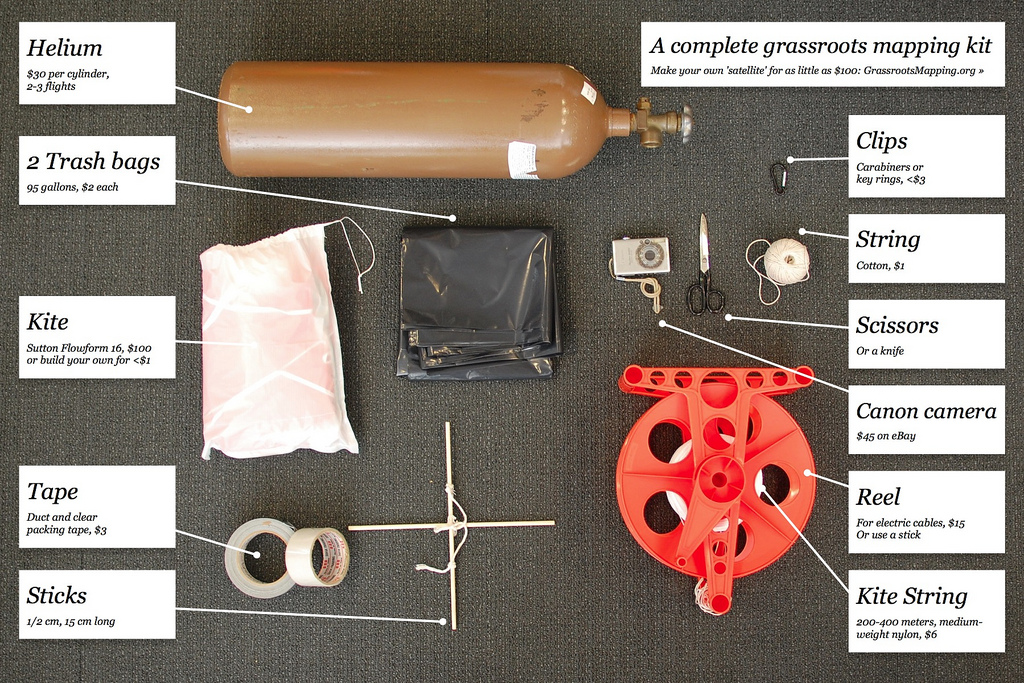
\includegraphics[width=0.45\textwidth]{images/100-dollar-satellite-poster.jpg}
	\end{flushright}
\end{wrapfigure}

\subsubsection*{Printed guides and support materials}
\subsubsection*{Curricular guides and teaching notes}

\subsubsection*{Documentation, case studies, Grassroots Map Collection}
\subsubsection*{The Grassroots Mapping community and mailing list}
\section{Novel Contributions}
\subsection{Novel application of low-cost tools to well-established need for raster imagery}
%\pdfcomment{do we discuss existing systems here? no, just mention paradigms of tiles, reference later section}

\subsection{Novel approaches to map rendering}
\subsection{Central merit: technology or culture?}
%both, duh: technology is only relevant in a context, and I make no attempt to separate this technology from its intended sociopolitical meaning

\chapter{Subjectivity in Mapping}

% text here, why is this chapter necessary:

The need for a more participatory cartography is predicated on the exclusion of many from the practice of map-making as it stands today. Even more importantly, it depends on the point of view that mapping is an inherently non-neutral practice, and that for maps to serve wider and more democratic interests, it must accommodate diverse viewpoints. Maps serve interests, and understanding their role not as documentation of what makes up the world, but as rhetorical, tactical, and \emph{subjective} tools is an important prerequisite to what this document argues.

\section{Neogeographers, Psychogeographers, and GIS}

A brief description of three distinct groups of practitioners is worthwhile, as each embodies a distinct conception of mapmaking. Each new 'generation' of mapmakers and mapping tools has positioned itself as a challenge to existing forms of cartography, and as such, the following will help to situate Grassroots Mapping and the Cartagen framework as another successive attempt to broaden participation and reconceptualize the practice. 

\subsection{Psychogeography}

Today, a variety of artists identify with the psychogeography movement, and continue to advance a contemporary take on the practice with new digital tools. These artists have in many cases successfully appropriated or even subverted geographic tools for a variety of causes. 

Examples from Radical Cartography and Experimental Cartography -- Proboscis, bodystorming, maps of indian territories, CUP, Sarai 

\subsection{GIS practitioners}

Professional map makers have used Geographic Information Systems, or GIS since its development in the 

% NEED reference for start of GIS practices - Qualitative GIS? 

GIS as a methodology has met with some criticism for its widespread use of expensive proprietary tools such as ArcGIS, both for their cost and because such tools present a high barrier to participation, 

... see Qualitative GIS ... criticism of GIS as a 'quantitative' tool ... 

A more recent offshoot of GIS is the Participatory GIS, or PGIS movement, which attempts to meet some of the criticisms of GIS by working with local communities as collaborators in the production of maps. 

\subsection{Neogeography}

With the rise of web-based data and display systems came a group composed primarily of programmers and web designers, who have adopted the name \emph{neogeographers}. This group positions itself in contrast to 'traditional' approaches such as GIS, and favors open data sharing, standards-based data formats, and free and open source software tools in place of proprietary solutions. The neogeographic movement, though it might have found its roots in the opening of the Google Maps API (see Chapter ), focuses today on largely web-based software such as OpenLayers, Mapnik, and GeoDjango. Some downloadable map viewing and editing packages such as QGIS or JOSM are also available, though even these are often used to produce data for web publication. 

One identifying theme in the neogeography movement is the shift of users from consumers to producers of maps. (Maps for Advocacy) The ability to create and publish map data using simple and free tools has dramatically broadened participation in map making, and Rana and Joliveau suggest that neogeography rejects the 'prescribed role/interaction between the four main components, namely the audience, the information, the presenter and the subject...'. \cite{rana2009neogeography} 

Another important aspect of the movement is that neogeographers typically do not come from a geography background, but from a programming and software engineering background. This has some technical benefits, in that the solutions they promote and develop are often conceived of from a different perspective, sometimes resulting in higher performance, broader applications, and reconcetualizations of both what and \textbf{for whom} maps are for. It has also resulted in an 'outsider' attitude amongst neogeographers, and even some resentment from traditional GIS practitioners; this has played an important role in how the movement presents itself to the rest of the world, and what choices it makes in the development of tools. For example, the OpenStreetMap project, discussed at length in Chapter 4, was developed in response to the restrictive copyright policies of the British ......... This has also led neogeography to share many of the goals of the PGIS movement, though relatively little communication exists between these two factions due to their different origins and mutually isolated venues for publication. (An exception is Mikel Maron's efforts in Kibera, among other places, which makes explicit reference to PGIS practices..... reference)

% the above needs reference... mikel maron

Andrew Turner: Introduction to Neogeography

\url{http://books.google.com/books?id=oHgDv4feV-8C&dq=neogeography+turner&printsec=frontcover&source=bn&hl=en&ei=gmDLS6_-KYj98AaY_KWXDA&sa=X&oi=book_result&ct=result&resnum=5&ved=0CBwQ6AEwBA#v=onepage&q&f=false}

"NeoGeography and the nature of geographic expertise", Author: Michael Goodchild  \url{http://www.informaworld.com/smpp/content~db=all~content=a911734343}
% goodchild-michael-neogeography.pdf

\section{The mythical `complete map'}

One common sentiment often heard in contemporary map literature is that the earth is more or less completely mapped. The availability of satellite imagery in tools like Google Earth, and the ability to zoom shockingly far into a dizzying array of places, from power plants in North Korea to the top of Macchu Pichu, gives the casual user the impression that we have indeed created a complete map of the world. However, if one attempts to find imagery of places which are removed \textbf{socioeconomically}, it becomes clear that while there may not be many \textbf{blank} spots on the map, there are an abundace of \textbf{blurry} spots. 

Illustration: Cities in Georgia, or Cameroon, or Bhagalpur, India.

This of course sidesteps the fact that an aerial image does not a map make -- in order to take advantage of the many applications of geographic data, vector maps, with labels, metadata, and routable relations must exist. These are almost entirely absent from many areas of the world (see Chapter 3). However, the fantasy that we have 'finished' is relevant to the attitudes....

A fictional version of this fantasy is mentioned in Lewis Carroll's \textbf{Sylvie and Bruno Concluded} on page 169. ... 'a mile to the mile!'
'So we now use the country itself, as its own map, and I assure you it does nearly as well.' p.169

This idea was later elaborated in a short story by Jorge Luis Borges and Adolfo Bioy Casares, called On Exactitude in Science:

\begin{quote}
...In that Empire, the craft of Cartography attained such Perfection that the Map of a Single province covered the space of an entire City, and the Map of the Empire itself an entire Province. In the course of Time, these Extensive maps were found somehow wanting, and so the College of Cartographers evolved a Map of the Empire that was of the same Scale as the Empire and that coincided with it point for point. Less attentive to the Study of Cartography, succeeding Generations came to judge a map of such Magnitude cumbersome, and, not without Irreverence, they abandoned it to the Rigours of sun and Rain. In the western Deserts, tattered Fragments of the Map are still to be found, Sheltering an occasional Beast or beggar; in the whole Nation, no other relic is left of the Discipline of Geography.
\cite{borges1946exactitude}
\end{quote}

Did I write this: The idea that maps accurately, or even completely depict a location is not entertained in a literal sense, yet amongst

Critique of quantitative GIS - Marianna Pavlovskaya, Non-Quantitative GIS, Qualitative GIS

% Title: UK Motorways 100% Complete
% I'm pleased to announce that the main carriageways of all mainland UK motorways have been completed.  Over 3,000 km of roadway.
% Etienne Cherdlu Sat Jan 7 10:45:05 UTC 2006

\begin{wrapfigure}{r}{0.5\textwidth}
	\begin{flushright}
		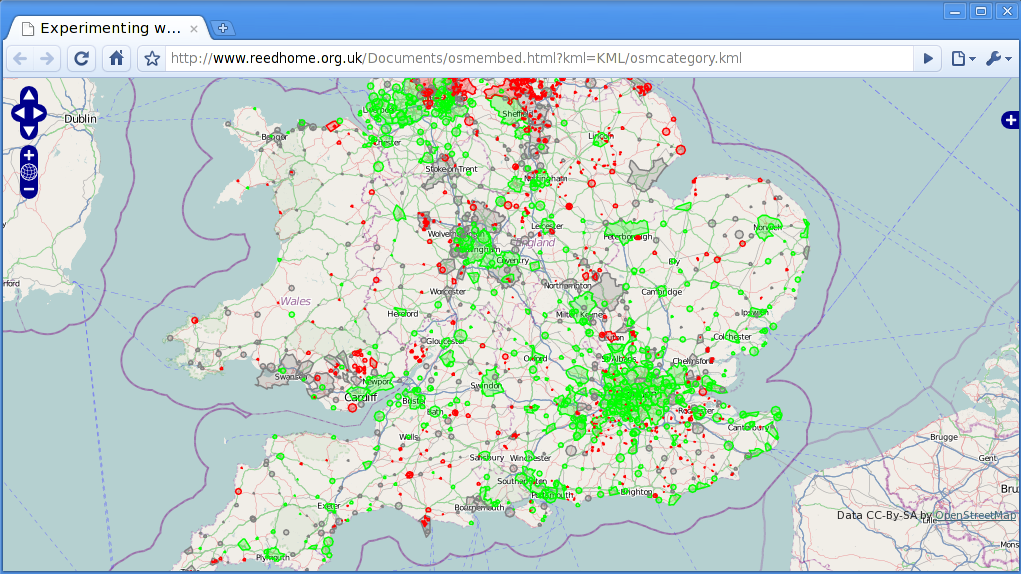
\includegraphics[width=0.45\textwidth]{images/osm-missing-parts.png}
	\caption{\url{http://www.reedhome.org.uk/Documents/osmembed.html?kml=KML/osmcategory.kml}}
	\end{flushright}
\end{wrapfigure}

Chris Anderson 

%We often imagine 'complete maps'
% Epistomology and mapping: maps are a form of technology, and of power      
%  - OSM reference to a 'complete map of UK'
%        - Chris Anderson's Wired article of complete dataset
% "At the petabyte scale, information is not a matter of simple three- and four-dimensional taxonomy and order but of dimensionally agnostic statistics. It calls for an entirely different approach, one that requires us to lose the tether of data as something that can be visualized in its totality. It forces us to view data mathematically first and establish a context for it later."
% Read More http://www.wired.com/science/discoveries/magazine/16-07/pb_theory#ixzz0lTiRSTXp
% rebuttal: http://www.edge.org/documents/archive/edge248.html#hillis
\section{Maps as a 'window' onto the world}

% essentially epistemological issue.

For a variety of reasons, maps carry the weight of authority in a way that few other forms of evidence do; the main driver being the widely held belief that satellite or aerial maps are a kind of 'window' into the world. In photography the editorial role of the author is accepted, not to mention the damage which 'photoshopping' has inflicted on the perceived truth or even objectivity of the photographic image. Maps, however, continue to be taken as direct representations of reality, desipte the inherent subjectivity of image selection, color, brightness, and contrast processing, and the editorial eye necessary in reading and interpreting such imagery. 

\begin{wrapfigure}{r}{0.5\textwidth}
	\begin{flushright}
		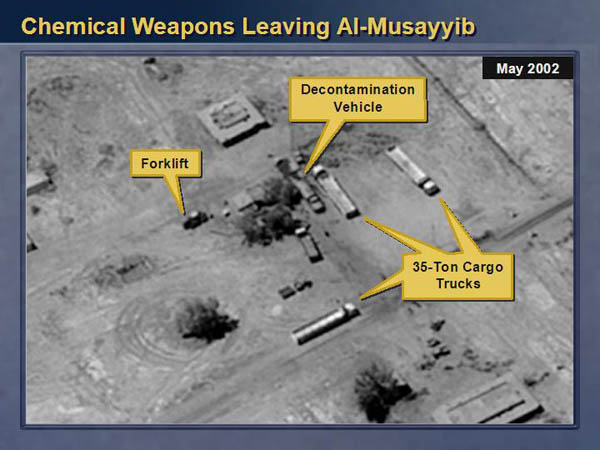
\includegraphics[width=0.45\textwidth]{images/iraq-image-16.jpg}
		\caption{\url{http://www.gwu.edu/~nsarchiv/NSAEBB/NSAEBB88/}, Image 16: Chemical weapons leaving Al-Musayyib}
	\end{flushright}
\end{wrapfigure}

The best example of this attitude is of course the use of relatively low resolution satellite imagery by Colin Powell at the UN Security Council in February 2003, used as evidence to support the existence of weapons of mass destruction in Iraq. The subsequent complete absence of weapons did little to diminish the public's faith in such imagery as objective evidence. 
% citation http://www.un.org/apps/news/storyAr.asp?NewsID=6079&Cr=iraq&Cr1=inspect

\begin{quote}
``Let me say a word about satellite images before I show a couple. The photos that I am about to show you are sometimes hard for the average person to interpret, hard for me. The painstaking work of photo analysis takes experts with years and years of experience, pouring for hours and hours over light tables. But as I show you these images, I will try to capture and explain what they mean, what they indicate to our imagery specialists.

...

How do I know that? How can I say that? Let me give you a closer look. Look at the image on the left. On the left is a close-up of one of the four chemical bunkers. The two arrows indicate the presence of sure signs that the bunkers are storing chemical munitions. The arrow at the top that says security points to a facility that is the signature item for this kind of bunker. Inside that facility are special guards and special equipment to monitor any leakage that might come out of the bunker.

The truck you also see is a signature item. It's a decontamination vehicle in case something goes wrong."
	\cite{guardian2003powell}
\end{quote}

\begin{wrapfigure}{r}{0.5\textwidth}
	\begin{flushright}
		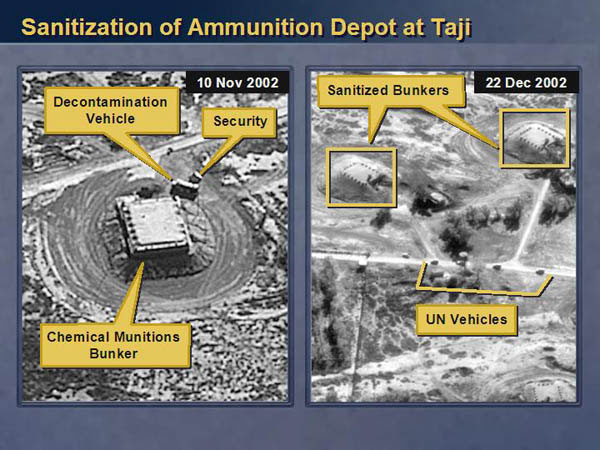
\includegraphics[width=0.45\textwidth]{images/iraq-image-13.jpg}
		\url{http://www.gwu.edu/~nsarchiv/NSAEBB/NSAEBB88/}, Image 13: Sanitization of Ammunition Dump at Tajii	
	\end{flushright}
\end{wrapfigure}

\begin{quote}
	``-- 10-11.***/WEAK. We support much of this discussion, but we note that decontamination vehicles--cited several times in the text--are water trucks that can have legitimate uses. A safer characterization is, `a vehicle used for chemical weapon decontamination.`

-- 11.***/WEAK. We agree there has been suspicious activity [redacted], including presence of a decontamination vehicle. We caution, however, that Iraq has given UNMOVIC what may be a plausible account for this activity--that this was an exercise involving the movement of conventional explosives; presence of a fire safety truck (water truck, which could also be used as a decontamination vehicle) is common in such an event."
	\cite{senate2004report}
\end{quote} 

% Fallacy!!! Wood, p. 20,21 - centimeter accuracy gives false impression of 'scientific accuracy' and completeness

What is most alarming about this kind of rhetorical use of map imagery is that it represents a means for those in a position of power to assert truths about places they have never been, without the involvement of human testimony from those who have.

This aspect of the public perception of maps as an objective, quantitative measure may have a relationship with the difficulty and expense of producing map imagery, and the traditional monopoly of government and high-tech industry in the production of such imagery.

\section{Maps: rhetorical, even tactical}
%        - Endless variety of possible data: Wood, Power of Maps, p.1
%        - not a representation of truth, but a rhetorical tool; Wood, p1?
%            - social construction of maps
% 	- map of sewer system from Wood
%	- Tactical cartography from Institute for Applied Autonomy
%	- http://www.tacticaltech.org/mapsforadvocacy
\section{Ground Truth, or maps as testimony}
%    - varying definitions of ownership, contested terrain
%        - 'Ground Truth' policy in OSM (http://wiki.openstreetmap.org/wiki/Disputes#On_the_Ground_Rule)

\section{Cartographic ethics}

In light of this reassessment of the political and social roles of maps and their production, some from the PGIS community have called for a code of ethics in participatory mapping projects. This seems especially prudent given that the production of maps can have dramatic effects on the residents of the mapped area. Giacomo Rambaldi, Robert Chambers, Mike McCall, and Jefferson Fox proposed in 2006 a set of 33 guidelines entitled "Practical ethics for PGIS practitioners, facilitators, technology intermediaries and researchers". The following is a sampling:

\begin{quote}
- Do your best to recognise that you are working with socially differentiated communities and that your presence will not be politically neutral
- Consider using spatial information technologies that can be mastered by local people (or local technology intermediaries) after being provided sufficient training
- Be considerate in taking peoples' time
- Stimulate spatial learning and information generation rather than mere data extraction for outsider’s analysis and interpretation
- Ensure that the outputs of the mapping process are understood by all those concerned
\cite{rambaldi2006practical}
\end{quote}

These guidelines demonstrate an belief that maps should be produced \textbf{in collaboration with} local communities, and with respect for their needs and interests. They have proved invaluable to the author in formalizing and understanding his interactions with mapping participants. In particular, they address the core concern of who owns the maps and for whom they are made; there is often the implicit assumption by enthusiasts of open geodata that simply dumping map data into OpenStreetMap is the end goal. It is important to be aware that most people (and especially those in communities in geographic conflict) are unaware of the existence of OpenStreetMap, and would likely be unreceptive to its benefits. 

Robert Chambers in particular warns PGIS practitioners against raising expectations of concrete results, noting that ``Any process of analysis facilitated by an outsider is liable to raise expectations of some benefit, even when the outsider goes to pains to explain that they have nothing to offer and nothing will follow from their visit. Disappointment, and reinforced disillusion with visitors and organisations outside the community then follow."


% email exchange from PPGIS list from early June 

% THIS WHOLE SECTION SHOULD PERHAPS BE MOVED TO 'DISCUSSION', post-Peru, or just after introducing state of the art... it may be a whole chapter.

Outline of history and benefits of PGIS, but also of ethics and beneficiaries

\subsection{Subjective cartography in practice}
%    - ref. West Bank mapping in Dec 2009
% Tree symbolism
% B'Tselem map of settlements
%        - mapping as testimony of use/presence/ownership by Abed's farm

\chapter{The Need for Geospatial Data}
\section{Two worlds of mapping}

Present-day users of web-based mapping products such as Google Maps are presented with an extremely rich cartographic landscape when they view maps of first-world urban centers such as New York and San Francisco. Real-time traffic data is often overlaid in lines of shifting red and green, and many buildings appear in orthographic '3D'. Well-known restaurants are interspersed with subway stops whose schedules may be called up with a few clicks. Routing algorithms offer turn-by-turn directions, optimized for pedestrians, bicyclists, and motorists. 

\begin{figure}[h]
	\begin{center}
		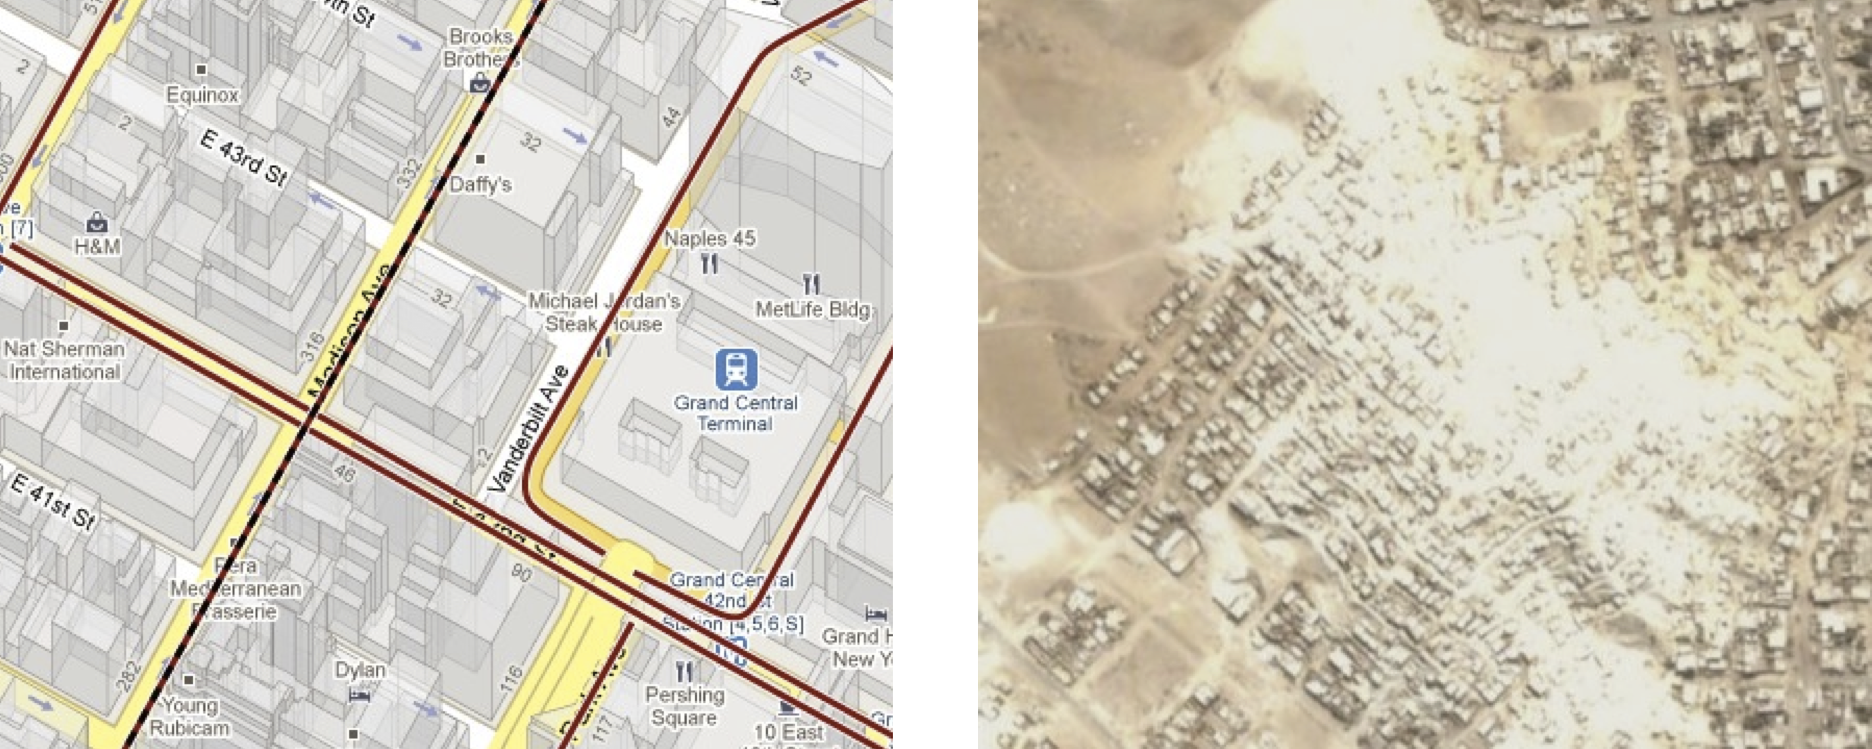
\includegraphics[width=1\textwidth]{images/two-worlds-mapping.png}
		Views of Manhattan, left, and a settlement in Lima, Peru, right, as seen in Google Maps \url{http://maps.google.com}
		% could add Cameroon, where towns are missing
	\end{center}
\end{figure}

Many are surprised when they view places such as Lima, Peru, a metropolis of 11 million people, and find that not far from the city center are vast areas of indistinct and unlabelled buildings. While some of these are recognized and official parts of the Municipality of Lima, many are informal settlements, whose inhabitants lack deeds to their plots of land, and whose streets and buildings do not appear on any city map. Many of these settlements, or 'invasions' as they are known to Peruvians, are governed by leaders who are either elected by the several hundred inhabitants, or who maintain control through intimidation -- employing thugs to collect taxes and enforce rules. 

A legal process exists to establish official land ownership in these settlements, and to issue deeds to their inhabitants, but the state lacks the resources to quantify or map these areas:

``...slums - all variety of precarious settlements - represent the `invisible' city, often omitted from official maps and documents and frequently physically hidden by local authorities by colorful walls and fences." -- `Slums of the World', UN-HABITAT, 2003

%    UN-HABITAT quotation
%	- “geographical mapping techniques to support struggles for social justice in India”. The end result, it added, could make maps as “tools to fight injustice in society”.
%	- http://timeoutbengaluru.net/aroundtown/aroundtown_feature_details.asp?code=59

In Lima, the organization in charge of land registrations, known as COFOPRI, requires residents to submit a plan -- essentially a measured and drawn map of their plots -- as one of many prerequisites to receiving a deed. Civil engineering firms have filled this gap by offering surveying and mapmaking services, but their high prices are a strain on the already poor inhabitants of the invasions.  

% find COFOPRI def
% image of posters showing what families owe to registration process

The Grassroots Mapping project was conceived as a means to broaden access to mapping technology, and was developed in direct response to the need for maps in informal settlements on the outskirts of Lima, Peru.

...

\subsection{Urban slums, informal settlements}

This state of affairs is not limited to Lima; by some estimates, a full quarter of the worlds population lives in urban slums. 

% find reference
% UN-HABITAT quotation

\subsection{Tenure mapping}

\subsubsection{The invasion of Lima, Peru}
%        - El Otro Sendero

The history of urban growth in Lima over the last hundred years can be described as a slow legitimization of vast areas of informal settlements; many populous and well-established districts such as Pamplona, Villa el Salvador and others, began as invasions decades ago.

Hernando de Soto, a well-known economist and champion of capitalism, ... quotation

Brief outline of fulfilled needs: chambers-who-empowered-disempowered-gains-loses.pdf, p.4
%            - graph of informal settlement percentages
%        - COFOPRI

\subsection{Mapping: a tool of empowerment or control?}

\begin{quote}
...it's frankly the same security through obscurity argument peddled for centuries, brought out most recently in Mumbai, a strategy on the verge of finally dissolving in a world of openness and transparency. The IDF access to much better intelligence and imagery than we'd ever have, they fly drones over Gaza, there's a 2m resolution commercial limit in all satellite imagery over Israel — guess who gets to see the sub-meter imagery? Gazans have nothing to gain by trying keep secrets, the asymmetry of that game is overwhelmingly not in their favor.\cite{maron2009misconceptions}
\end{quote}

\begin{quote}
In general, I view these edge cases as a question of power. Hiding information protects those already in power, but not those that are already marginalized. Legitimate cases to me is only information that puts dis-empowered people at risk, such as refugee routes along the Burmese-Indian border.\cite{maron2010freedom}
\end{quote}

Evgeny Morozov, "How dictators watch us on the web" - \url{http://www.prospectmagazine.co.uk/2009/11/how-dictators-watch-us-on-the-web/}
\url{http://irevolution.wordpress.com/2010/01/07/morozov-vs-shirky/} (Patrick Meier)

many criticisms may represent limited experience mapping... circular?
It is easy for activist cartographers who do not live in a community to advocate the use of tools which may put that community at risk.

"empowerment":(great article on definitions for empowerment and framework for discussing empowerment in the PGIS context)

Corbett, Jon M., and C. Peter Keller. 2005. An Analytical Framework to Examine Empowerment Associated with Participatory Geographic Information Systems (PGIS). Cartographica 40 (4):91-102.

\section{Environmental assessment}

Beyond issues of land rights and ownership, there are many other potential uses for inexpensive map data; the ability to produce photographic, or raster maps of sensitive environmental sites may empower small organizations which are unable to acquire timely or high resoultion satellite images of sites of interest. One case study we will examine is that of a group of environmental activists in West Virginia who have struggled to gather meaningful and quantitative evidence of the environmental damage and health hazards of mountaintop removal mining across the Appalachia region of the United States. Besides the prohibitive cost of traditional satellite imagery and high level of expertise required by traditional GIS tools, they strive for data which will make a visceral and emotional impact on policymakers and regulators, as well as the general public. 

Among other metrics, they make use of water conductivity tests to determine the degree of contamination due to runoff and blackwater releases. Conductivity is a secondary measure, and is not as direct as photography. Aerial imaging, or specifically mapping, is an ideal blend of direct measurement and visual appeal, and its main detractor is its price; overflights cost hundreds of dollars each and image processing is labor- and skills-intensive. A case study examining the applicability of Grassroots Mapping tools to this problem was performed in May 2010 and is discussed in Chapter 12.

\subsection{Asset allocation mapping and carbon cowboys}

\cite{poole2006there}

%	- bibliography/poole-peter.pdf
%	- stewardship of biodiversity, p.2
%	- case study uses of mapping capability, p.5
%	- detecting and monitoring impacts of industrial-scale development

\section{Open geodata and crisis mapping}
\subsection{Crisis mapping and Ushahidi}

A variety of different sorts of 'crowdsourced' or grassroots mapping strategies have evolved in recent years with the intent to respond to, document, analyze, and report on the real-time occurrence of disasters and crises. From environmental crises such as the April 2010 BP Oil Spill in the Gulf of Mexico to the humanitarian crisis in the aftermath of the January 2010 Haitian earthquake, a clear need has evolved for low-cost, decentralized situational awareness and documentation tools with geospatial features. Here we discuss some of the challenges of fulfilling such diverse needs under unpredictable conditions.

\subsubsection{Ushahidi}

The Ushahidi platform has emerged as a common and easy-to-install system for crowdsourced crisis reporting. Developed in collaboration with Kenyan programmers to help voters report election violence in Kenya in 200x, it allows citizens with mobile phones to send 140 character text messages to a publicized telephone number.\cite{okolloh2009ushahidi} These messages are read by a group of editors, who attempt to identify where the messages were sent from, and are published on a web site as red dots at their assumed location. That users self-report their locations, and can do so incorrectly, is tolerated because it may represent a means of privacy for users, and because in the aggregate it is quite difficult to 'fake' an event. Each report is 'verified' by ... 

% ref. AJ Turner's presentation at Where 2.0, i think - or Patrick Meier's on iRevolutioni
% interview LABB folks about how reports are verified

Ushahidi works in many cases because it is simple to understand on its surface; visitors to an Ushahidi web site see a series of dots with messages such as "I'm stuck under rubble" and imagine a person sending such a message from their cell phone. It makes use of existing communications infrastructure, namely that 'most people have cell phones' and relies on both a high level of literacy with text messaging and a willingness to send reports to a site which is not immediately viewable. However, it is not a means to 'make' a map, but rather to annotate an existing map with data points.

Ushahidi has been successfully used to gather and publish very up-to-date information about unfolding crises, for example in the instance created by the New Orleans-based environmental group Louisiana Bucket Brigade in response to the British Petroleum oil spill in April 2010. The kind of information it provides, however, is fundamentally difficult to verify or to quantify, and may be more useful in the context of emergency response than in evidence-gathering. Locations must often be approximated to the nearest town or city, and most reports are often just a few words with no name or photographic evidence. While geotagged photographs can be uploaded to Ushahidi, EXIF data can be falsified. In many cases there is an additional need for quantitative data. Map imagery provides better quality information in that every pixel of a map is georeferenced.  

\subsubsection{Photographs and maps as testimony}



\subsubsection{Satellite imagery}

Public access to up-to-date imagery of crisis areas has become something of a hot-button issue in crisis mapping circles, as those companies and agencies in control of the imagery do not always elect to release it, or to license it freely for any use. Whethe due to an unwillingness to offer expensive imagery for unrestricted use, or due to the administrative burden of actually offering such data for download under a permissive license, access to satellite imagery has become a frequent bottleneck for aid organizations. 

Specifically in the bottom-up response to the Haitian earthquake and subsequent humanitarian crisis of January 2010, access became more difficult within weeks of the crisis. While GeoEye and other vendors generously offered open access to satellite imagery in the initial weeks of the crisis, most did not elect to do so on an ongoing basis, or for subsequent crises such as the February 2010 earthquake in Chile.



% Republishing Christiaan's response or UN-SPIDER's response may not be allowed, depending on the policies of the Crisis Mapping Network

% who released data??? 

Mikel Maron of the OpenStreetMap Humanitarian Team 

%	- origin in political mapping, focus on natural disaster
%        - UN-SPIDER/Google MapMaker response to Mikel Maron, Chile Earthquake

\chapter{State of the Art}
\section{PGIS: Participatory Geographic Information Systems}

Traditional GIS technology has been used for since the 1990's to support communities in developing contexts for purposes such as making tenure claims, environmental defense against petroleum and other extraction industries, as well as for planning purposes. This has become known as PGIS, or Participatory GIS, and typically... 

% See Peter Poole's Life after Tenure Mapping for a brief historical timeline, i think



PGIS was part of a more general movement towards a ``critical GIS" practice, which could . Sarah Elwood summarizes various alternative GIS movements, one which ``could incorporate diverse forms of spatial knowledge and promote multiple epistomologies" \cite{elwood2009representations}

``how GIS, spatial data, and maps produce and negotiate politics and power relations, or how they can be used to foster participatory decision making processes."

\begin{quote}
It was also in 1988 in an AKRSP (India) RRA training involving Jennifer McCracken, Anil Shah, Parmesh Shah and others, that a headman, asked to present to the villagers the map the outsiders had draw, had difficulty until he turned it ``upside down", which was the way he and the villagers saw their village . . . . We were teetering on the brink of learning that ``They can do it".
\cite{chambers2006participatory}
\end{quote}

\subsection{PPGIS}

Definition: \url{http://www.ppgis.net/ppgis.htm}
Bibliography: \url{http://dusk2.geo.orst.edu/gis/student_bibs/slurie.htm}


bibliography/rambaldi-participatory-spatial-developing-countries.pdf

\subsection{Participatory GIS for Development}
% Jen Osha's article
%\href{http://www.directionsmag.com/article.php?article_id=2365&trv=1.}{Participatory GIS - A Paradigm Shift in Development?} - Jen Osha and Daniel Weiner, 2006
%        THE ILLUSTRATED GUIDE TO NONPROFIT GIS AND ONLINE MAPPING: http://maptogether.org/nonprofit-mapping
%        Claudia Canepa's PhD dissertation
\subsection{Shortcomings of traditional PGIS practice}
%    Peter Poole - Life after Tenure Mapping
%        - outsourcing of GIS processing typical, problems

\section{Web mapping}

Some degree of mapmaking has become commonplace to the internet-connected public since the advent of highly user-friendly `slippy map' interfaces such as Google Maps. This has been especially true since the release of the Google Maps Application Programmer's Interface (API) in the summer of 2004, allowing programmers to modify and repurpose Google's web map services.  Early examples of reuse included the GMaps Pedometer, which would output the linear distance of a path you walked, along with how many calories you burnt. \cite{gibson2006google} From the frivolous to the essential, this means of mapmaking has become widespread and relatively easy. However, many would argue that this is not mapmaking at all; most of the users of Google maps do not edit the underlying map data, but overlay points, lines, and polygons \textbf{on top of} Google's proprietary data.

\subsection{Google Maps and proprietary data}

In fact, not only Google Maps, but the vast majority of the online maps are based on the relatively static base maps made available by larger organizations. Google and other providers of map data publish these maps as collections of small image 'tiles'; JPG or PNG images of typically 256 by 256 pixels, which are rendered ahead of time and cached. These are served using Apache or another conventional web server. The main benefit of this technique is that it serves map data as a set of common image files; a standard and highly optimized means of distribution. These are re-assembled in the browser into a seemingly continuous map, and as the user pans or `slips' around, new tiles are transferred to maintain the illusion of a continous map.

A second reason for the use of map tiles is that it is quite difficult to reconstruct the original discrete vector data set from map tiles; in this respect they are similar to compiled code. Google and other commercial map vendors do not share their point, line, and polygon data, nor do they make metadata such as labels or land use markers available. Distributing tiles gives them a degree of control over what source data they choose to release, and allows them to maintain control of those assets.

Distributing the underlying data used to generate these tiles conflicts with these companies' business models: such data is valued intellectual property. The tile-based rendering system strips the map of its metadata, making a local, or personal, critical, or revisionist interpretation quite difficult. Tiles immutable – they contain no information about authorship, no hyperlinks, and in order not to crowd a given tile, each one displays only a selection of available data for that corresponding area of the world. 

\begin{wrapfigure}{r}{0.5\textwidth}
	\begin{flushleft}
		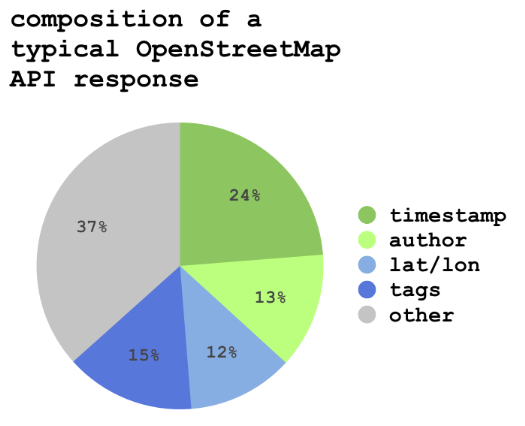
\includegraphics[width=0.45\textwidth]{images/osm-composition.png}
	\end{flushleft}
\end{wrapfigure}

Open data projects such as OpenStreetMap, the 'wiki map of the world', do just the opposite – like the open source software projects they took inspiration from, they share the entire dataset as coordinates, semantic tags, polygons, and most importantly, time and authorship data. In the case of OpenStreetMap, anyone with enough disk space can download the entire planet's worth of data (over 200 gigabytes when loaded into a database) and create their own maps. In that dataset in particular, authorship data actually outweighs its geometric counterpart. Perhaps even more tellingly, historical data – for areas of the map which have been overwritten – occupies more storage space than current data. This suggests that authors have challenged each others' data more than they've added new data to unmapped areas. \cite{warren2009composition}

\section{OpenStreetMap}

OpenStreetMap.org, taken as an open-source software project, a database of open geodata, and a community of volunteer mappers, represents one of the best examples in recent years of the \textbf{neogeographic} response to PGIS. That is, without explicit ties to the PGIS movement, or even a high degree of literacy in the movements 2 decades of literature and research, OpenStreetMap (or OSM, as it has become known in neogeographic circles) has attempted to meet many of the same goals. OSM encourages volunteers around the world to contribute to a single, shared digital map and corresponding map database. 

In many ways it has met with wild success, and the size and detail of the OSM map database is formidable. 
% How big is it? 
However, participants are overwhelmingly European and American, and tend to be wealthy due to the emphasis on internet connectivity and the use of GPS devices to produce new map data.

In fact, the OSM data collection strategy relies most heavily upon three sources. First, existing municipal and public domain databases make up an enormous part of the available data; the TIGER database produced by the US Census increased the size of OSM by a factor of ten. Second, tracing of satellite data with the Potlatch, JOSM, and other tools to extract vector data from rasters plays a large role, especially in areas with few local participants. This technique was used in the OSM Gaza project to map all of Gaza using a satellite dataset purchased for \$5,000 from donations during the Gaza war in late 2008. \cite{maron2010openstreetmap} While convenient in that it does not require mappers to actually travel to the places they are mapping, it does not actively involve residents of an area in the mapping process, and sufferes from many of the shortcomings which inspired the PGIS movement. 

Finally, much of the OSM database was created by individuals carrying GPS devices to record GPX tracks, or collections of latitude/longitude coordinates. These are later uploaded, annotated and merged into the main OSM database using tools such as JOSM. This is the preferred means of collecting data because of its high accuracy, its emphasis on firsthand mapping, the clear legal ownership of the data, and because of the implicit belief among many OSM participants that better maps are made `on the ground'. 

This belief is supported by the `on the ground' policy stated explicitly in the OpenStreetMap wiki, a central organizing document of the community.

\begin{figure}[h]
  \begin{center}
    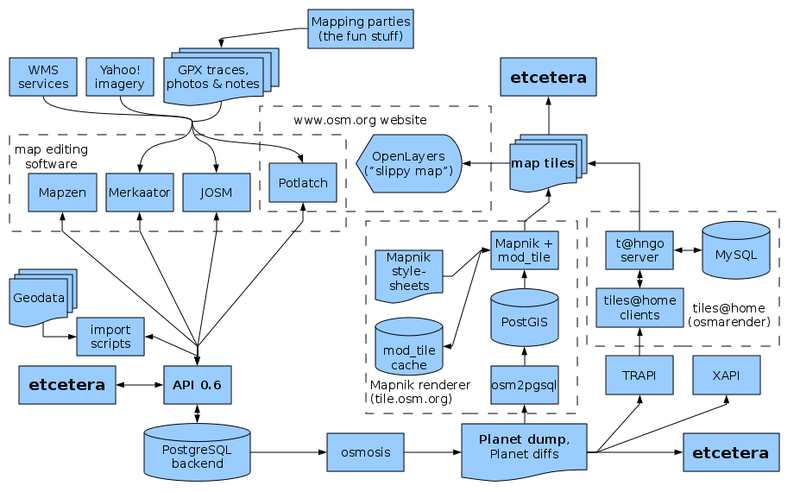
\includegraphics[scale=0.45]{images/osm-diagram.png}
  \end{center}
\end{figure}

\subsection{The modern open-source geostack}

Another interesting aspect of OpenStreetMap is that it represents a deployed and working combination of many of the premier open-source mapping tools available today. It makes use of OpenLayers, a web browser-based framework for displaying raster map tiles using JavaScript. Tiles are produced using Mapnik, the popular open-source tile renderer. An array of other open-source utilities are used to create, edit, translate, import, and export the data. 

...

\subsection{Humanitarian OSM Team}
 
An offshoot of the OpenStreetMap project known as the OpenStreetMap Humanitarian Team or HOT was started in late 2009 by Mikel Maron, a map programmer and co-founder of mapping firm Mapufacture. Positioned in direct response to the need for maps in areas of humanitarian crisis, Mikel has organized members from the technology community to visit crisis zones such as Port-au-Prince as well as a long-term presence in Kibera, a large slum in Nairobi, Kenya. HOT uses the same tools as the wider OpenStreetMap community, and either runs a separate instance of the OpenStreetMap server and database, or directly uploads the data to the main OpenStreetMap.org service. 

\url{http://wiki.openstreetmap.org/wiki/Humanitarian_OSM_Team}

\subsubsection{OSM Gaza}

HOT's first project, a volunteer effort to map the Gaza Strip during the 2008-2009 war between Israel and Gaza, relied on Yahoo Maps and Digital Globe satellite imagery. Over seven days, OpenStreetMap volunteers traced the satellite imagery in order to produce a more accurate, more up-to-date map, and with assistance from JumpStart International, the map was available online and for download with no copyright restrictions. This emphasis on placing map data (not just rendered maps!) in the public domain was intended to provide for the widest possible uses of the information, on both a technical and legal basis. In order to preserve this legal status, the OSM Gaza dataset was published separately from the main OpenStreetMap database, though in accordance with its liberal licensing, a copy was uploaded to OSM as well. Building on the success of the OSM Gaza project, HOT went on to collaborate with a variety of organizations in countries like India, Kenya, and Georgia, all using the OpenStreetMap toolset. 

\begin{figure}[h]
  \begin{center}
    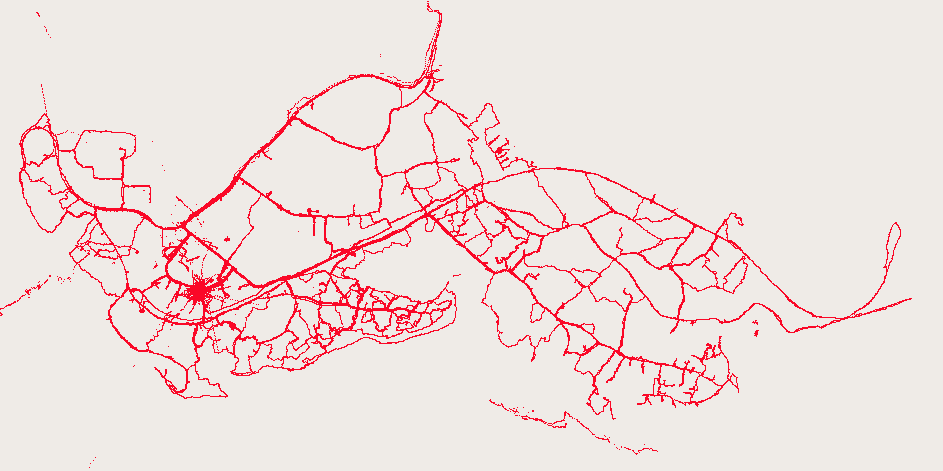
\includegraphics[width=1\textwidth]{images/kibera-gpx.png}
    GPX traces collected from GPS units over three weeks of mapping in Kibera. \url{http://www.flickr.com/photos/mikel_maron/4143021346/}
  \end{center}
\end{figure}

Two projects by HOT stand out as their most ambitious and influential. The first, called simply Map Kibera, produced a map of the famous Kibera slum in Nairobi, Kenya, in collaboration with several local organizations. This project differed from earlier HOT projects in that it relied primarily upon local participants using hand-held GPS units to produce the map, as well as with paper-based annotations using the Walking Papers system developed by Michal Migurski of Stamen Design. With a specific mission to engage with the sociopolitical aspects of cartography, Map Kibera is much more explicit than OSM Gaza in its agenda and the needs it addressed. It also represented a shift away from remote mapping by means of tracing, towards a model which relied more heavily on local expertise and familiarity with the site. In this sense it has much more in common with the Grassroots Mapping project; both attempt to empower local communities by buildling local capacity and ceding control over the mapping process to local individuals and organizations. 

The second project of note is the map making work done in the aftermath of the January 2010 earthquake in Haiti.

\begin{quote}The have been at least 400 OpenStreetMap editing sessions in Haiti since the quake hit. Mostly tracing Yahoo imagery, and gleaning information from old CIA maps. We also just received permission to use GeoEye imagery acquired post-event … that will allow us to tag collapsed buildings.\end{quote} \cite{maron2010haiti}

\begin{quote}`Sea change in the legitimacy of crowdsourced geographic data. For instance, all the United Nations agencies acting on the ground in Haiti used OpenStreetMap for their print maps'\end{quote} \cite{glennon2010grassrootscrisis}

%        Data modeling: http://wiki.openstreetmap.org/wiki/Humanitarian_OSM_Tags/Humanitarian_Data_Model
\subsubsection{Challenges}
%        Slum mapping, disaster-specific issues
%        architectural/infrastructural shortcomings
%	reliance on GPS, or need for a base layer
% 	inclusion in a GPS-device process
%	ease of use, black-boxing of information
%	JOSM, other issues with typical deployment
\textbf{Emphasis on local infrastructure}

\section{Existing techniques for low-cost orthorectification}

While there are a diverse range of approaches to participatory mapping, several prior works have focused on free or widely available tools for orthorectifying aerial imagery as a means to produce and publish mapping data. Their uses range from stitching aerial imagery captured from hobby-levelremote control aircraft to rectifying historical printed maps in order to digitize their contents.

\subsection{Map Warper}

Perhaps the most ambitious project of this type is the Map Warper software written by Tim Waters, Schuyler Erle, and Shekhar Krishnan, as part of their project to 'crowdsource' the digitization of the New York Public Library map archive. \cite{waters2009warper} The tool, built for the New York Public Library Map Archive to digitize their collection, invites volunteers to orthorectify maps by matching Ground Control Points, or GCPs, between a source image and a reference map. 

While designed for warping archival maps onto a vector dataset, namely OpenStreetMap, the tool can be used to warp aerial imagery onto satellite data. This is achieved by inserting a new layer into the reference map pane, which is implemented in OpenLayers. The resulting warped image can be downloaded as a GeoTiff or accessed as a standards-compliant WMS layer. 

\subsection{GonzoEarth and manual stitching with Adobe Photoshop}

One of the main practitioners of low-cost mapmaking today is Stewart Long and his one-man company GonzoEarth. Stewart is responsible for such impressive maps as the 2009 map of Burning Man, published at a 3 cm resolution. This map was surprisingly warped onto a lower resolution base map, blended, and output as a BigTiff image using Adobe Photoshop CS4. The image was then reprojected and saved as a GeoTiff using the open source GDAL package.

The imagery for the Burning Man map was taken from a balloon by ....... , but Stewart typically uses a lightweight and relatively inexpensive remote control airplane called the Easystar, sold by the German company Multiplex. A small canon camera is inserted into the cockpit and a hole is cut in the belly of the plane through which the pictures are taken. Stewart can fly the plane at up to a half-mile away, steering manually with a 2.4 Ghz transmitter and can capture imagery at hundreds of feet in the air. The plane can remain in the air for up to an hour. 

Reasons... get quotation

DIYDrones T3

% mention DIYDrones, kite aerial photography guy with hugin/big Xs on the ground 

\chapter{Grassroots Mapping as an alternative means of participatory cartography}

How do the tools/technologies outlined above meet the needs described, and how are they better?

%    Meet subjectivity needs
%        - against a canonical datastore
%        - solution lays in tools and formats and practices, not in a single project/datastore
%            - therefore GM & Cartagen are based around:
%                - a body of code
%                - a thorough documentation and guide to mapping techniques
%		- a series of case studies
%        - options to organize project: as a 'generic hub' for imagery, like OpenAerialMap, engage primarily via internet/blogs
%            - or, focus on collaborating with specific communities in cartographic dispute
%                - expand into matchmaking between mappers and communities in need, as well as supporting via mailing list 
%                - maintain open communication with end-users, iterate back into tools: 
%                    - requests made via list: stewart long asks for masking, Crispen asks for entry of lat/lon pairs, WhereCamp folks asked for locking, Pat Coyle asked for 'natural_size' feature

\section{Aerial imaging with low-cost tools}

Due to the need for cheap and up-to-date imagery, a major part of the Grassroots Mapping project has been the design and use of low-cost platforms for capturing images of the ground from above. The use of kites and balloons to raise consumer-level 'point-and-shoot' cameras has allowed participants to capture images of sites of interest at minimal cost. A 'Grassroots Mapping Kit' can be assemnbled for less than \$100. 

\begin{quote}
In parallel came the discovery that local people could readily interpret black and white aerial photographs, often at 1:5000 (Dewees 1989; Mearns 1989; Sandford 1989). 
\cite{chambers2006participatory}
\end{quote}

\section{Cartagen: an alternative architecture for digital maps}

However, in order to orthorectify or `stitch' aerial imagery into a flat, geographically referenced map requires a system to display and manipulate raster imagery. The ability to label, trace, and otherwise annotate the resulting rectified map requires a system to display and manipulate vector data. In order to meet these needs the author created a map authoring and display framework called Cartagen. Written in JavaScript, it enables users to edit and publish discrete map data (points, lines, polygons) using a text editor, and to view and manipulate that data in a modern web browser such as Safari, Chrome, or Firefox. Maps may be published in just a few flat files, rather than relying upon a tile caching system or a backend database.

raster abilities of Cartagen

Beyond the ability to orthorectify imagery, Cartagen is a fully-fledged cartographic scripting environment and renderer. It can draw vector data onto a pixel grid - not just fast enough to generate tiles, but at over 10 frames per second on most computers. As the user interacts with a Cartagen map, features are drawn continuously, as in an animation. This negates the need to cache or otherwise store raster representations of map data, and sidesteps many of the assumptions and limitations of the modern mapping technology stack.

This alternative `geostack' is one of the most unique aspects of the Grassroots Mapping tool chain. Far from an unnecessary reinvention of the wheel, the abilities it affords make it suitable for deploying original data without placing a high demand on technical skills or resources. 

Reference chapter 4.2 discussion on current geostack 

%        - existing solutions based around cloud systems
%            - this move opposite - closer to client
%            - needs: data under no connectivity
%            - multiple devices
%            - ownership of data/infrastructure
%                - FrontlineSMS, 'local' is a feature, opposite of corporate/commercial strategy
%        - low-AI approach; technical literacy, flexibility, admits 'misuse'
%            - examples: USGS overlay at WhereCamp 2010
%            - additon of non-map features with Warper tool
%            - difficulty of use of hugin, etc
%                - DIYDrones thread: "3 days stitching and tweaking images" (http://diydrones.com/profiles/blog/show?id=705844:BlogPost:134855&page=1#comments)
%            - Stewart Long uses Photoshop for most stitches (get him on record)
%Emphasis on building in response to end-user needs
%    - this work could only be done by working with communities in cartographic dispute. See Lima case study.

\chapter{Related works}

Additional non-technical works?

%    Inspiration, context, history of activist/grassroots mapping
%    Reiterate HOT/Free Map Palestine, India, Kibera
%    GroundTruth, Jai Sen, A People's Atlas of Chicago
\section{Beyond symbolic mapping: Data-driven approaches to participatory mapping}
%        Expanding role of mapping to legal, tactical
%        Institute for Applied Autonomy

\chapter{Evaluation criteria}

In assessing the Grassroots Mapping project, I wanted to consider not only the technical merits of the tools and their immediate use, but the success of the project as a human endeavor, and in terms of its effects on the communities involved. While there are important quantifiable benefits to the balloon- and kite-based techniques for capturing imagery and the web-based tools for processing and publishing that imagery, it is also important to address the degree to which the tools were appropriate for participating communities, and whether they felt that the tools served their needs. 

\section{Participants vs. collaborators}



%        Role of Carla, Escuelab, Shuawa
%        Hector as a fellow educator (interview)

\section{Openly ideological research}
%    'Reconceptualizing Validity' (Patti Lather, p.67)
Critique of quantitative GIS - Marianna Pavlovskaya, Non-Quantitative GIS, Qualitative GIS
\subsubsection{Triangulation}
\subsubsection{Construct validity}
how theory was affected by data
\subsubsection{Face validity}
how research was received by participants
\subsubsection{Catalytic Validity}
how participation transforms the situation (self-awareness/reflexivity)

\subsection{Interviews with local partners}
Wiki, mailing list, blog, media coverage (~ Face validity)

\section{Comparison with existing techniques}

% possible table of comparison... based on Stewarts?

One of the most compelling aspects of the balloon and kite mapping techniques was its low cost; many of the communities I worked with, including those in Canta Gallo, Lima, and Rock Creek, West Virginia, mentioned cost in particular as a motivation to try these tools. For volunteers at the Louisiana Bucket Brigade in New Orleans, it was the low cost of a mapping kit which made it possible to scale up mapping efforts to several teams, with new maps made every few days, all within a budget of only a few thousand dollars.

Compared to the alternatives, of hiring pilots and paying for fuel and aircraft, or purchasing satellite imagery, balloon and kite mapping seemed not only inexpensive, but more legible and participatory. The idea that one would have to send a camera into space to photograph things which are right next to oneself seems strange, especially when the area of interest is on the scale of a small community. Imagery taken from only 2-4000 feet preserves a sense of the human scale; mappers can often see themselves or their boat or car in the images, and the occasional photograph shows the balloon or kite string leading down from the camera to the ground. This leaves a powerful impression on mappers, who are literally holding the camera in their hand at thousands of feet in the air... albeit at the end of a string. To them, the millimeter-thick string is both a literal and symbolic link to the camera, a reminder of their control over the image and the authorship they have in the resulting map. 

In pragmatic terms, rather than relying on an outside source of expertise, members of participating communities felt that they could perform the image collection themselves, at times of their choosing, and could repeat the imaging at higher intervals than what would be possible with aircraft or satellites. After performing several 'trips' with members of the Louisiana Bucket Brigade and members of Coal River Mountain Watch, participants from those organizations felt comfortable launching their own balloons under observation by myself or Stewart Long, another grassroots cartographer. Several of these participants went on to lead their own trips and bring back their own imagery.

\section{Quantitative evaluation}

\subsection{Resolution}
 
On a purely technical basis, there were several key benefits to to the techniques employed by the Grassroots Mapping project. In terms of resolution, 

\subsection{Time}

Though \textbf{some} satellite imagery is publicly available for virtually every place in the world, and often at useful resolution, even those areas which are mapped at better than 1 meter resolution are often years out of date. The ability to \textbf{repeatedly} image an area at intervals of one's choosing makes balloon and kite mapping techniques useful for time-sensitive purposes such as periodically monitoring the effects of the Gulf oil spill (see Chapter 10) or measuring vegetative regrowth in mountaintop removal mining sites undergoing reclamation (see Chapter 12). 

\subsection{Color}

Aerial imagery taken from low altitutdes (under 4000 ft) typically has better color saturation and more spectral information is preserved compared to imagery captured from space or from higher altitude aircraft platforms. This can be significant for environmental assessment, as is the ability to get uncompressed RAW format image data; Crispen Wilson of Conservasi, a  member of the Grassroots Mapping mailing list, is attempting to do spectral analysis of aerial imagery over water. Most aerial or satellite imagery is published as PNG or JPEG tiles, and is not useful for such purposes.  

% back this up... spectrum preservation and altitude
% histogram illustrations


\chapter{The Grassroots Mapping tool chain}
\section{Balloon/kite Aerial Mapping (BAM/KAM)}

previous BAP/KAP for mapping: Eric Wolf, others
 
\begin{wrapfigure}{r}{0.5\textwidth}
	\begin{flushright}
		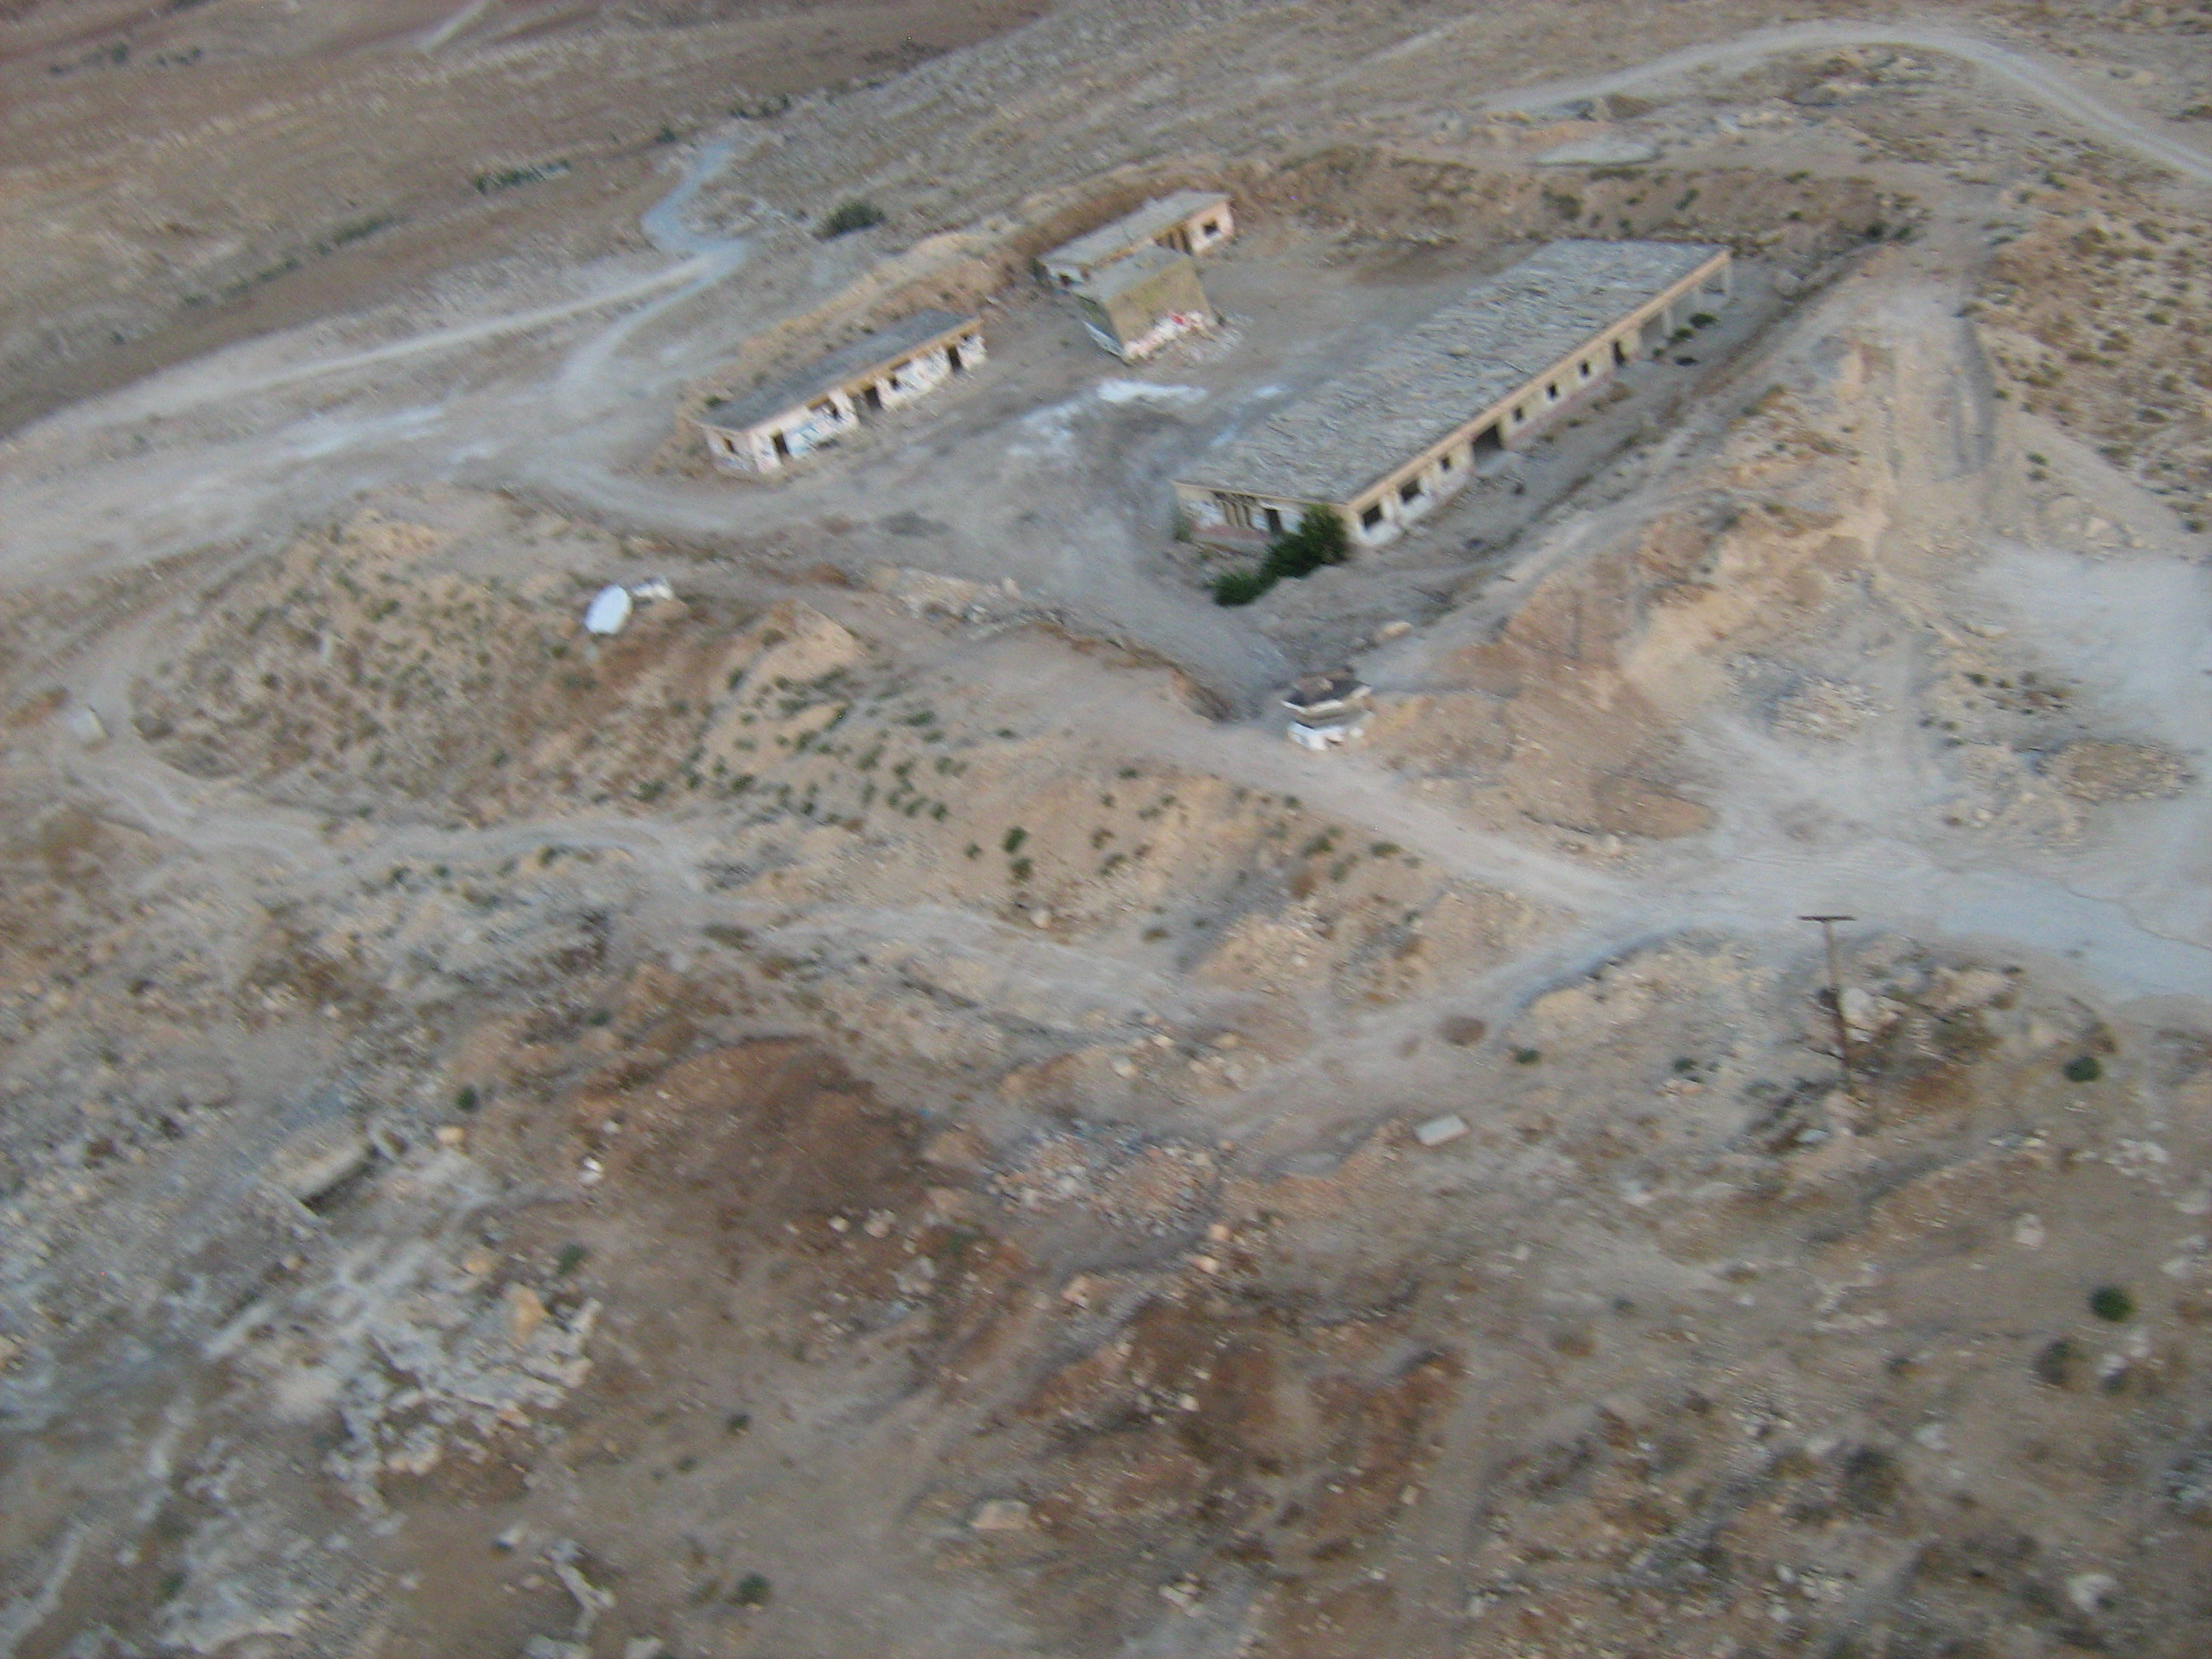
\includegraphics[width=0.45\textwidth]{images/maron-spy-satellite.jpg}
		\cite{maron2008former}
	\end{flushright}
\end{wrapfigure}

%    UAV - DIYDrones and collaboration (see 'Future work')
%        Leveraging both expert and 'amateur'/enthusiast expertise
%        Connecting hobby/DIY communities with activist communities and agendas
\subsection{Accuracy and precision in kite and balloon imaging}
% focus on cost goals, 'mapping at all'
% Eric Wolf's thesis on BAP metrics: wolf-eric-thesis.pdf

\section{Digital maps: reconceptualizing mapping interaction}

Once aerial imagery is captured, software must be used to distort or 'warp' the photos and combine them to fit a projection. This essentially maps every pixel of the source imagery to a position on the earth's surface, allowing for correlation to other maps and geodata sources. As no existing tool met all of the design requirements, such as cost, ease of use, low barrier to entry, and performance (see Chapter 9), I developed a unique tool and associated mapping framework with the goal of making DIY cartography simpler, cheaper, and more inclusive.

\subsection{Cartagen dynamic rendering}

As discussed in Section 4.2, most digital maps today employ a server-side caching mechanism providing a tiled image collection. The tiles are assembled seamlessly in the user's browser, and zooming is accomplished by maintaining multiple tilesets -- one for each zoom level. The resulting system scales predictably, as tiles do not vary dramatically in file size, and can be served using Apache or even stored locally. While this works well for a single dataset such as terrain contours, it commits the map to a single representation. Multiple tile sets can be stacked, and polygons can be overlaid, but most importantly, the user cannot edit the tiles or manipulate the data they contain. Compressing data into tiles strips them of their metadata and authorship information in favor of scalability and consistency. 

Diagram of Cartagen vs. Existing geostack

To sidestep many of these requirements, and to allow users to participate fully in the authoring of maps, I created the Cartagen framework. Using new techniques made possible by widespread browser support for HTML5 and specifically the Canvas element, Cartagen can create maps which are not pre-rendered, but generated on-the-fly. This frees the map from a single projection or representation, and enables a more dynamic, interactive, and narrative cartographic style. Discrete vector data (made up of points, lines, and areas) can be downloaded in JSON format just once, and displayed at any scale and in any style. Recent increases in JavaScript execution speed [JavaScript speed stats] make possible relatively high framerates (~15fps on a typical machine), obviate the need for browser plugins like Flash or Java, and make dynamic HTML5 mapping accessible even on mobile devices such as on the iPhone, Android, and Windows Mobile platforms. As an added advantage, Cartagen performs much of the work of map display locally, reducing dependence on high-latency internet connectivity. It also allows users to easily download data and view or edit it offline. These features make it particularly appropriate for use in developing countries or in crisis situations. 

Wiley's Last Resort image

The Cartagen framework represents an alternative system which is optimized for user-created content, rather than one-to-many broadcast publishing. As a fully scriptable cartographic environment, however, it was also uniquely suited for building an image orthorectification tool. The Canvas element is essentially a pixel raster, but because Cartagen's primitives are vector objects stored as points and polygons, it there is no need to store resampled source imagery while performing distortions or transforms. While in Photoshop, a powerful computer is required to store, manipulate, and export a map of any considerable size (maps made for the BP oil spill project were over 50,000 px in each dimension), Cartagen can be used to orthorectify using a laptop or even a low-power netbook. Users in effect see a lower-resolution preview rendered only at the size of their browser window, and a final, high-resolution composite image is created using ImageMagick on the server side. This lowers the cost of the equipment to process and orthorectify aerial imagery by thousands of dollars. 

%            Existing vector systems (Chris Schmitt's email on geowanking)

%                GSS (and OSM-JSON): appropriating the HTML/CSS paradigm for data legibility and open access
%                    Format politics: XML, JSON, RSS

Despite reinventing much of the typical geostack, Cartagen makes use of open standards such as JSON, OSM-XML, and GeoJSON, and can be used to generate GeoTiffs or even a TMS tile service. In addition, because it can store and display both raster and vector data, once images are rectified, the pen tool can be used to trace streets, buildings, and borders.   

Another unique part about Cartagen is that it allows users to style vector map data using a stylesheet, in a syntax similar to that of CSS. This is intendd to mirror the content vs. style relationship between HTML and CSS, and in fact the map stylesheet format Cartagen uses is called GSS. This is intended to leverage the widespread literacy in web design and provide a scaffolding for those just beginning to make their own maps with these tools. 

Illustration of GSS

\subsection{Why an entirely new mapping system?}

needs rewrite for thesis style:

In a sense, rendering is at the heart of the argument for critical cartography. If mapping is to be a means to advance an agenda, or develop a narrative, or create a communal self-image, it must allow for diverse forms of representation. We have the divergent data and the means to collect, collate, and publish it – what we lack is a way to represent it in layered, interactive, and radically unique ways. 

Cartagen is distributed solution to the problem of generating complete world maps with minimal resources, which describe a constantly changing data set. This turned out to be both technologically advantageous and epistemologically transformative. Once maps are rendered in your browser window instead of by Google or Yahoo, you are empowered to design, manipulate, and use that data in new and compelling ways. 

Instead of just annotating a Google Map with pins representing your data, Cartagen provides an opportunity to create your own map from scratch, using both open geodata and data you've collected from your environment. Mapmaking with Cartagen is a form of cartographic narrative. 



\subsection{Beyond raster mapping/Tile politics}



%            Metadata: authorship data
%            Google Maps png metadata hack
%            GIS and broadly adopted consumer-focused mapping stacks

\subsection{An iterative toolchain development process}

Important to the development of the Grassroots Mapping tools was a collaborative process of testing various tools in a variety of contexts. Various combinations of tools were tested with participants from Lima, Peru, New Orleans, and Rock Creek, West Virginia. Verbal and interview-prompted feedback was used to develop new tools which built on the strengths of existing and off-the-shelf systems such as Photoshop, Hugin, and Map Warper. The same is true for the physical tools such as the balloon and kite kits, including the camera housing, reel construction, and auto-triggering setup. 

Shots from Pat Coyle's demonstration

In the case of the camera housing, Grassroots Mapping community members have iterated and improved upon the soda bottle enclosure, discussing and testing alternatives on the mailing list, and even posting videos of tests. Pat Coyle, a mailing list member, published a narrated demonstration of a soda bottle enclosure with improvements such as a window to access the camera controls and a small bungee cable to stabilize the camera against the inside of the bottle. In another example, Mathew Lippincott prototyped solar-powered hot air balloons constructed from painter's plastic sheeting, conducted pigmentation and lift tests to determine suitability for carrying cameras. The tests and builds were held at a public event in Portland, Oregon, and the resulting balloons were packaged and sent to New Orleans for use in the BP oil spill mapping (see Chapter 10). 

Illustration of Mathew Lippincott's workshop 

Regular testing of new tools at the MIT campus, as well as repeated attempts to orthorectify the resulting imagery, grounded the software development in concrete usage and experience, and a workshop at the Google campus in Mountain View in April 2010 included a collaborative hacking session aimed at identifying and resolving bugs and adding new features in direct response to the day's mapping efforts. 

Imagery from Google hacking session

\subsection{Web-based orthorectification and warping}

In response to the collaborative design process and interviews conducted in Lima, Peru (Chapter 9), it was determined that the primary barrier to producing map imagery was the orthorectification process. While in Lima, participants made use of Adobe Photoshop CS3 as well as the Map Warper software discussed in Chapter 4. Attempts were made to instruct residents of the subject areas in the use of these tools. These techniques met with limited success due to factors such as availability of computers powerful enough to run Photoshop, latency in internet access, and most of all, the obscure interfaces which users were required to learn (see discussion in 9.1.9).  

Using Adobe Photoshop to manually disort and warp imagery over an imported base map was a more direct and easier to explain process, but the low availability of the software and the need for a powerful computer to perform large image transformations were additional challenges. The need for a lightweight, easy to use system became clear. The additional ability to run such a program in any standard web browser would put such tools within reach of anyone with access to an internet cafe.

\subsubsection{Cartagen Knitter}

The Cartagen Knitter software, developed in the months following the Lima, Peru mapping project, makes this possible. Using the Cartagen Framework along with an HTML 5 distortion technique prototyped by Steven Wittens of acko.net \cite{wittens2008projective}, the author created an interface for users to upload images as overlays on an existing base map (typically OpenStreetMap vector data) and to manually distort an image by dragging the corners with the cursor. Tools for rotating, scaling, and adjusting the transparency of images were created, and the tool was tested and refined in a variety of workshops and mapping projects over several months. 

Cartagen Knitter makes several unique choices about how users rectify imagery. The first is that it emphasises orthorectification of individual images against a base map, rather than initial stitching of images into a larger composite image, then subsequent orthorectification and warping of that larger image. This decision was based on the relatively high computing resource requirements of manipulating a single higher-resolution image, given Knitter's emphasis on low-resource usage. Additionally, Eric Wolf of the US Geological Survey has found experimentally that the composite, or mosaic, technique suffers from a loss of accuracy: 

\begin{quote}
"The process of creating a single mosaic from the images and then geo-referencing wholly to the USGS High Resolution Imagery resulted in a reduction in accuracy of nearly 100\% in both location and orientation"
\cite{wolf2006lowcost}
\end{quote}

The second design decision which may seem curious is the emphasis on a completely manual orthorectification interface: no automated interest point finding or matching is used, despite the availability of such software (i.e. Hugin, Photosynth, Vision Workbench, etc.). Even Map Warper (reference) automatically warps images, though it asks users to identify common Ground Control Points to determine how to perform the warping.

- didn't do a good job
- very difficult to configure
- high resource requirements
- tended to exclude participants from process



\chapter{Case Study: Grassroots Mapping in Lima, Peru}

\section{Introduction}

In the interest of basing tool development and design on real-world applications, and due to an ongoing conversation with Carla del Carpio of Lima-based Manzanita "A", the author travelled to Lima, Peru in January 2010 to work with several informal communities and NGOs on mapping projects. From the start, this was considered an experimental program, where Peruvian collaborators would help to better define needs and to iterate and improve upon the balloon- and kite-based imaging techniques.

The program was also explicitly educational in its goals, and with educators from Lima-based Centro de Información y Educación para la Prevención del Abuso de Drogas (CEDRO) and Manzanita "A", a curriculum was developed to involve local youth in the mapmaking process. An emphasis was placed on examining the cartographic process with students not only in the sense of recording the present layout of students' communities, but with the intent to depict and discuss the past and future of the communities. A series of exercises were devised to situate mapping as a way to examine and reflect upon dynamic, growing communities.

Because of the land-ownership situation discussed in earlier chapters, the Lima project was also intended to provide easy and inexpensive alternative means for communities to produce maps specifically for tenure claims. However, the author and members of the partner NGOs felt that this agenda should be secondary to the educational goals. Further discussion cemented their belief that as non-residents who would not be affected by the outcome of more political and legal uses of the maps, it was not their place to aggressively advocate such uses. 

\subsection{The Other Path: Lima's history of informal settlement}

Lima, Peru was chosen as an ideal pilot location in part because of the author's familiarity with local NGOs and the development community, however the city's unique history made it an especially good choice. Lima has expanded over the last century to include a full third of the population of Peru, in what has become a process of continuous and transformative growth. The result is a city in which large tracts of land have been settled 'extralegally', a term borrowed from Hernando de Soto's exhaustive history in `The Other Path'. These settlements are known locally as `invasions' due to their inhabitants' sense of having not only literally seized the land from private landowners or the government, but of having unilaterally constructed a working alternative to the official municipal government, including public works, tax collection, and education. These communities, typically made up of only a few hundred people each, are truly apart from the central government, and only through a years-long process are able to gain title to their land along with basic services such as plumbing and electricity.

De Soto paints a picture of a government entirely overwhelmed by the floods of immigrants from rural areas, and entirely unable to accommodate these newcomers in its infrastructural or bureaucratic capacity. ``We appear to be witnessing", he writes, ``the most important rebellion against the status quo ever waged in the history of independent Peru." The stunning statistics of the informal population; he describes in detail how "...through invasions or illegal aquisitions of land, neighborhoods sprang up which today account for 42.6 percent of all housing in Lima and are home to 47 percent of the city's population." \cite{desoto1987sendero}

This context, though not unique in the world, is especially appropriate as a place to attempt a mapping project which acts outside of traditional cartographic means of production, and outside the conventional framework of GIS. In the months that followed the Lima project, the author began to refer to the tools and techniques which were prototyped in Lima as a kind of `DIY satellite', and that seems fitting given that in the invasions of Lima, residents are accustomed to Doing Everything Yourself, from constructing roads to building and maintaining their own plumbing. In addition, any means to reduce the barriers to acquiring tenure is held in high value; de Soto holds that ...
%        - de Soto's work; tenure 9x value

\subsection{Designing tools with, not for, participants}

Both Manzanita ``A" and CEDRO were enthusiastic about the potential of a mapping project from the outset, and Carla del Carpio coordinated with CEDRO's Ernesto Fernandez to set up a Projecto Integral
% define a Projecto Integral
with a group of approximately a dozen students in the Juan Pablo II settlement in Lima's Villa el Salvador district at the south end of the city.

Emphasis was placed on collaborating with local NGOs such as CEDRO and Manzanita ``A" rather than in the roles of researcher and subjects, or even designer and client. Decisions 

Initial discussion established several possibe use cases for maps, such as demographics to 

..support planning by NGOs, infrastructural assessment...  
.. see Maps for Advocacy for uses, also Practical PGIS...er, the blue reading

\subsection{Valuation and 'grey' economies}

%        - asset mapping; NiJeL, informal economies

Many invasions are self-governing, and elect a group of 'dirigentes' or leaders in charge of specific tasks, such as public works. According to Manzanita "A", one of the main roles of the leadership of an invasion is as record keepers for land ownership; even in the absence of state-sanctioned deeds, plots are allotted to families. However the ability to transact land sales or to leverage one's plot as collateral for loans is dramatically increased upon receiving title. 

p. 24, value of buildings with title 9x that of buildings without - also expectative property right and evolution of title

\subsection{Limits of state-sanctioned mapping efforts}

%        - COFOPRI and history of ineffective state-led mapping/legalization processes
%    Current approaches to mapping: 
%        COFOPRI, engineering firms, comparisons with OSM-HOT, UN-SPIDER from earlier discussion

\subsection{A Grassroots Mapping curriculum}

As planning progressed for the month-long Projecto Integrador, it became clear that much of our preparatory work was laying the foundation for a youth curriculum in participatory mapping. The group felt strongly that beyond simply producing a map, the activities should include a discussion of the political and social role of cartography. This was elaborated in a series of loosely-planned exercises which broke up the regular kite- and balloon-flying activities. 

\subsection{Mapping with Juan Pablo II}

%            - CEDRO & Manzanita "A"
%            - size, ages, of kids
%            - outline of activities
%                - (Illustration of timeline)
                - Introduction to mapping
                    - discussion: literal mapping difficult due to different mental models
                    - tape-measure technique -- bodystorming
                    - introduction to Google imagery not relevant
\subsubsection{First flights in Juan Pablo II}

%                - Initial balloon flights
%                    - technical issues
%                    - difficulty in involving kids in process
%                        - note: thought about potential for each student to build a satellite: want to try
%                    - immediate interest & success amongst community members

\subsubsection{Situating mapping practice}

%                - Printing & review of images
%                    - unanticipated interest in seeing selves from above
%                - History & Future exercises
%                    - Having seen community from above made representation easier
%                    - interspersed with flights
%                    - very specific information about construction/infrastructure from Frank & others
%                    - maquette in 3D - unsolicited - wealth of specific information about goals
%                        - 3 story buildings (sendero - stored wealth/bank accounts)
%                        - explicit connection between mapping and urban planning
%                        - real engaging activity as a corollary to mapmaking
%                        - references to infant care (WaWaWasi), shops, flowers, soccer fields
%                        - Project Morrinho maquettes in Brazil

\subsubsection{Stitching maps with Juan Pablo II}
                - Stitching exercises
                    - with kids - 'rubber sheets'
                        - with teachers (secondary audience) - Map Warper, discussion of difficulties (see ahead)

\subsection{Mapping with San Ignacio Loyola}
% (have title and survey)
            - Manzanita "A"
            - usage of Photoshop primarily; fast mapping; 2-3 hrs flight, 1-2 hrs stitching
            - Hector: ideal user: 
                - lives in an informal settlement
                - teacher, interested in using this in curriculum
                - community leader
                - interest in tech, willing to try map warping
                    - difficulty in trackpad/menu usage, took notes
                - engaged despite workload
                - sees applicability for mapping tools in settlements

\subsection{Mapping with Cantagallo}
            - Escuelab - technology, art, society
            - engaged with a creative group, Shuawa
\subsubsection{The Shipibo in Lima}
            - narrative of 10 year stay, claim to land, contested claims, and riverbank site
            - Escuelab sought political neutrality, but obviously interested in political situations: ex: shipibo language            - Drawing exercises
                - 'amazon' home vs current home
                - non-literal mapping - related to issues of veracity re: Wherecamp sugg. of children mapping with stickers
\subsubsection{Flying balloons with Cantagallo}
- fastest yet
                - total images
                - usage of hugin/SIFT/Photoshop
\subsubsection{Lower Cantagallo and local geographic dispute}
            - Escuelab and Sara/CEDRO
	- two cantagallos (three?)
            - Sr. Ricardo - possible political engagement/entanglement
            - entry into SETAME site; playfulness seen as neutrality? Or just no resistance at low levels to mapping activity?
                - not perceived as claim-related?
	- ``De hecho hasta ahora no hay uno mejor que el tuyo. En los demás mapas simplemente Canta Gallo no existe." - Helder Solari, one of the activists participating in the Escuelab/Canta Gallo collaboration

\begin{wrapfigure}{r}{0.5\textwidth}
	\begin{flushright}
		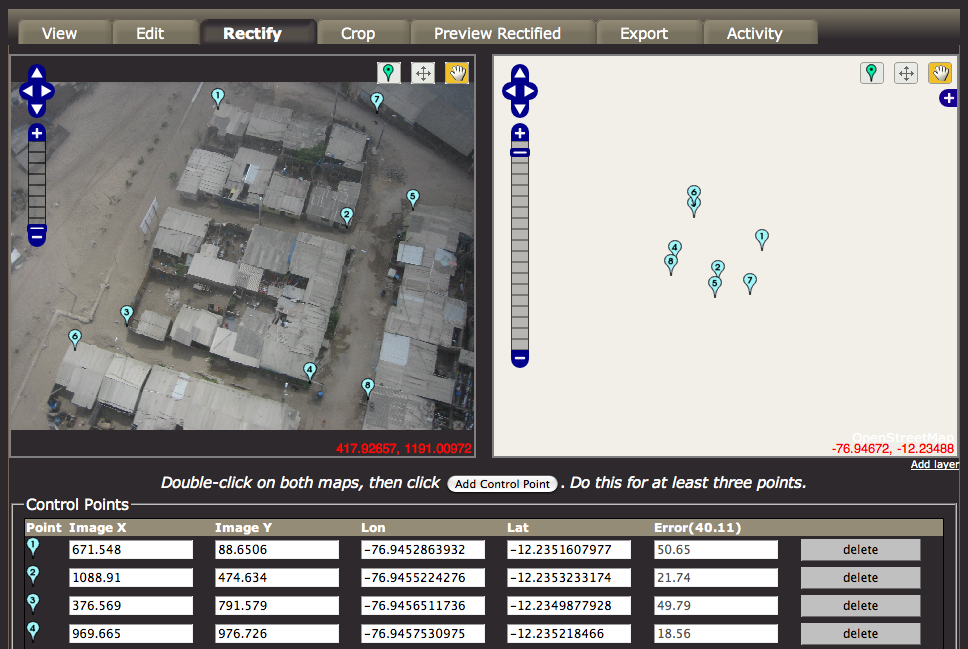
\includegraphics[width=0.45\textwidth]{images/map-warper.png}
		The Map Warper interface for identifying Ground Control Points. \cite{waters2009warper}
	\end{flushright}
\end{wrapfigure}

\subsection{Computing literacy challenges with orthorectification}
	- map warper
        - designed for printed maps
        - large loop of interaction - overcorrection easy, no immediate feedback upon assigning GCPs
        - difficulty in explaining GCPs, and necessity of javascript hack for areas without base data
        - amazing for intended use, even note application in Mumbai

\begin{wrapfigure}{r}{0.5\textwidth}
	\begin{flushright}
		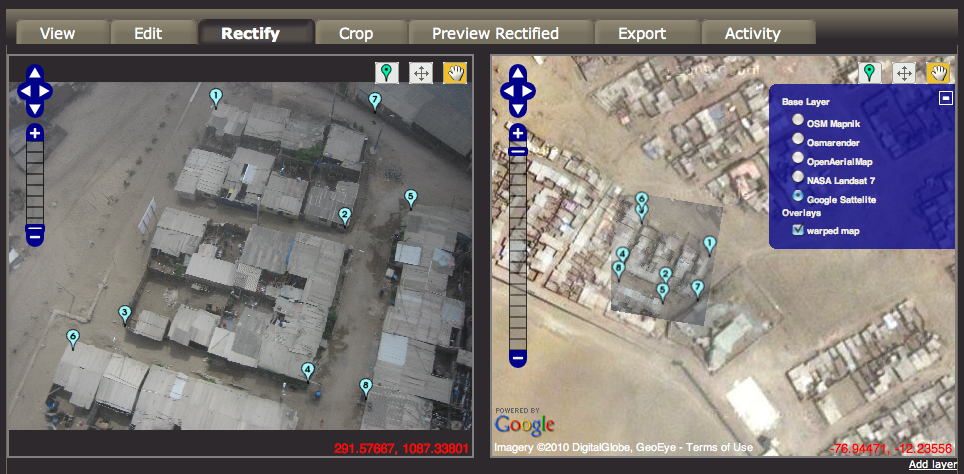
\includegraphics[width=0.45\textwidth]{images/map-warper-hack.png}
		Demonstration of JavaScript hack to insert Google satellite data for warping in areas with low feature density. \cite{waters2009warper}
	\end{flushright}
\end{wrapfigure}

    - Photoshop better, but barely
	- stuart long uses photoshop, maybe bruce owen (see emails)
	- ``For example, tracing was chosen over digitisation, and simple graphics software over geographic information systems (GIS)." \cite{poole2006there}
\subsection{Evaluation}
- based on criteria
        - Interviews!!!!!!! transcribe them
        - Applications of maps we made
            - legal role
            - import to OSM?
            - World Bank mandate to map every home? do we support that goal?
            - education, urban planning, NGO planning support, demonstration project
\subsection{Needs (Re)assessment}
- Goals for a true 'pilot' that goes beyond information gathering and use of existing State of the art tools
   - planning of new, easier interfaces and techniques
                - Map Warper difficulties, speed
            - discussion and 'designing with' leading to Cartagen Knitter (see later discussion)
		- http://en.wikipedia.org/wiki/Rubbersheeting
            - needs assessment - user-centric design, appropriate design
    - Possibility of mapping a fast-changing community
        History/future assignments make explicit the value of mapping as an activity

\chapter{Case Study: Citizen mapping of the BP oil spill}
\section{Grassroots mapping in crisis response}

In late April 2010, the Deepwater Horizon oil rig exploded and sank, initiating what may be one of the worst environmental disasters in US history. As the spill grew in size, the author contacted Stewart Long of GonzoEarth.org and Oliver Yeh of 1337arts.com. Long has used remote control aircraft to produce maps, and Yeh specializes in high-altitude photography using weather balloons, having captured imagery from a balloon at altitudes of over 90,000 feet. The three decided to travel to the Gulf Coast area to spearhead a citizen effort to map the oil spill's effects. After making phone contact with Anne Rolfes of the Louisiana Bucket Brigade (LABB), a New Orleans-based environmental activist group, Yeh and the author flew to New Orleans on May 5th 2010, followed by Long on May 6th. 
% env. crisis in US history: http://www.npr.org/templates/story/story.php?storyId=126410895
% http://www.nytimes.com/2010/04/25/us/25rig.html - Oil Leaking Underwater From Well in Rig Blast, By CAMPBELL ROBERTSON, April 24, 2010

With the cooperation and extensive support of the LABB and other interested New Orleans residents, the team began leading almost daily trips to use balloons and kites to map coastal areas. While not attempting to produce imagery of the entire at-risk coastline, which stretches several thousand miles from Louisiana to Florida, the mappers focused on acquiring high resolution imagery of specific sites, with the goal of producing 'before and after' maps. The trips relied on the availability of free transport to affected areas, but in the initial days of the project this was not a problem, as fishermen and charter companies began calling in to offer their services for free. Increasingly large areas of the Gulf of Mexico were being closed to fishing, and with their livelihoods at risk, many in the fishing industry were eager to participate in the documentation of the spill. 

% fishery closings: http://sero.nmfs.noaa.gov/deepwater_horizon_oil_spill.htm 

The 2010 Gulf oil spill was seen as an opportunity to apply the low-cost mapping techniques refined and documented on GrassrootsMapping.org to a problem of immediate import. While many overflights were occurring, there was no publicly available, orthorectified imagery available in the initial weeks of the spill; up-to-date imagery was supplied mainly by the MODIS (Moderate Resolution Imaging Spectroradiometer) sensors aboard NASA's Terra and Aqua satellites. MODIS is limited to 1000 meter resolution for those bands which are used for ocean imaging, and while the daily images available were very useful in determining where along the coast was being hit by slicks and sheens, it was not of high enough detail to show any specific damage. 

% http://modis.gsfc.nasa.gov/about/specifications.php

By contrast, the imagery collected by the LABB/Grassroots Mapping teams was up to 9 cm/px in resolution, and could be repeatedly captured over the course of days or weeks.  

In the first days of the 2010 BP oil spill mapping project, members of the Grassroots Mapping community worked with the Lafourche Port Commission and their contractors from Boston-based Priority5. 

\chapter{Case Study: A Grassroots Mapping curriculum in Georgia}

In early 2010, Jeff Haack of JumpStart International, the nonprofit group which funded and operated the Free Map Palestine project with Mikel Maron in 2008-9, expressed interest in applying Grassroots Mapping tools and ideas to a nation-wide mapping project in the country of Georgia. With educational projects in 5 cities across the country, this was to be the first large explicitly educational application of the Grassroots Mapping concept. Beginning in June 2010 and lasting 6 weeks, the program consisted of a series of workshops and trainings with JumpStart-affiliated educators and activists using balloons, kites, and remote controlled airplanes.

\begin{quote}The NGO structure JumpStart has built in Georgia is, in my opinion, an apt and sustainable way forward. After our experience in Palestine it became clear that impact requires a lasting effort in a community and the encouragement of local skills and ownership. It’s not merely about mapping a country, but about understanding where that, conceptually, meets societal needs, and building value therein. Sustainability for Open Maps Caucasus comes by understanding the convergence of digital technologies with community mapping, social fabric, governance, and civil society, and filling a need within that sphere. We’re not expecting OMC’s community mapping focus to last forever, but that concept, at the very heart of it is meaningful and sustainable, because accessing the tools for extracting and considering not oil or timber, but information, strengthens a society and can make it more prone to long term development.\end{quote} \url{http://brainoff.com/weblog/2010/04/28/1556}

\chapter{Project sustainability and ongoing work}

\section{Additional ongoing uses of Grassroots Mapping tools}

\subsection{Coal River Mountain Watch}

\section{Wiki, blog and mailing list}
        Incorporation of new needs through dialogue (see Evaluation Criteria .. Face validity/Construct validity)
        Examples of community-based reformulation/innovation
            Crispen's suggestion of lat/lon rectification points (mentioned above)
            Pat Coyle's videos, bungee-cable design, and camera shutdown research

\section{Illustrated Guides}

Originally suggested on the Grassroots Mapping mailing list in ....... by list member Pat Coyle, the idea of an illustrated guide to provide a rich and cross-language instruction set has received some attention. Storyboarding, outlining, and initial sketches were begun in the spring of 2010 by Pay Coyle, Nathan Cooke of MIT's D-Lab, 

Crispen Wilson or Peter Poole asked for a guide.... find the email

The 4-page PDF guide developed for the Louisiana Bucket Brigade was a quick attempt to provide such instructions, but was primarily intended to serve as an organizational guide and checklist, with tips and reminders, rather than a complete start-to-finish guide. 

\section{Outreach}

There has been a great deal of interest from both technology enthusiasts (kite, RC airplane, and geo-programmers alike) and organizations working in local communities to implement Grassroots Mapping tools and techniques. Part of the ongoing development of this community will be the brokering of relationships between these two communities, and the matchmaking of those with the technical know-how with those in need of geospatial information and training. The Grassroots Mapping mailing list incorporates representatives of both of these groups, and as such will continue to be the central organization point for such collaborations. I plan to organize meetup sessions in key areas to bring these communities together in a hands-on, workshop setting, where personal connections and professional relationships can evolve.

\chapter{ReadingList}

\hypertarget{related_readings_1}{}\subsection*{{Related readings}}\label{related_readings_1}

\href{http://www.unicef.org/teachers/researchers/intro.htm}{Curriculum on ``{}Children as Community Researchers''{}} - UNICEF, authored by \href{http://web.gc.cuny.edu/che/cerg/about_cerg/environmental_learning_index.htm}{Children'{}s Environment Research Group}

\href{http://www.directionsmag.com/article.php?article_id=2365&trv=1.}{Participatory GIS - A Paradigm Shift in Development?} - Jen Osha and Daniel Weiner, 2006

\href{http://www.iapad.org/pgis2005/}{Mapping for Change} - 2005 International Conference on Participatory Spatial Information Management and Communication

Weiner, D. and T. Harris, 2003. ''{}\href{http://www.rri.wvu.edu/pdffiles/gisweiner.pdf}{Community-Integrated GIS for Land Reform in South Africa}.''{} URISA Journal. 15(2): 61-73.

\href{http://books.google.com/books?hl=en&lr=&id=_VK-ABCKlVgC&oi=fnd&pg=PA3&dq=Nino+Bariola&ots=_r1wMwjiou&sig=TH0Gn1P27Xtsdq2Oc0Up5D6HLzg#v=onepage&q=Nino%20Bariola&f=false}{Bilingualism and identity: Spanish at the crossroads with other languages} - Geographic dispute in Canta Gallo, in Lima, \href{http://books.google.com/books?id=_VK-ABCKlVgC&lpg=PA3&ots=_r1wMwjiou&dq=Nino%20Bariola&lr=&pg=PA153#v=onepage&q=&f=true}{Chapter 7}

\href{http://www.sciencedirect.com/science?_ob=ArticleURL&_udi=B6VG2-4XHJX4B-1&_user=10&_coverDate=08/31/2009&_rdoc=1&_fmt=high&_orig=search&_sort=d&_docanchor=&view=c&_searchStrId=1186930669&_rerunOrigin=google&_acct=C000050221&_version=1&_urlVersion=0&_userid=10&md5=a9327ffa62e089e863f892a4551c1717}{Intervention: Mapping is critical!} - This intervention targets the much heralded demise of the map in geography and the recently proposed “rethinking” of maps. It comprises contributions from two political geographers, a military geographer, a political scientist, and two activist cartographers and argues that there is not so much a need to “rethink” maps, but to “re-engage” with the material practices of mapping, and above all to “re-make” maps.

\href{http://training.esri.com/campus/library/bibliography/RecordDetail.cfm?ID=95545&browseonly=0}{Mapping in a Shoebox} - A Grassroots Approach for Developing the Geospatial Literacy of Elementary Children - 24th International Cartographic Conference - Jaqueline M. Anderson, Sally Hermansen, Lorraine Innes, 2009

Lots of work by Proboscis: \href{http://urbantapestries.net/}{Social Tapestries/Urban Tapestries}, 2002-7 - Urban Tapestries investigated how, by combining mobile and internet technologies with geographic information systems, people could `{}author'{} the environment around them; a kind of Mass Observation for the 21st Century. Like the founders of Mass Observation in the 1930s, we were interested creating opportunities for an ``{}anthropology of ourselves''{} – adopting and adapting new and emerging technologies for creating and sharing everyday knowledge and experience; building up organic, collective memories that trace and embellish different kinds of relationships across places, time and communities.

\chapter*{Appendix A}

%%%%%%%%%%%%%%%%%%%%%%%%% BIBLIOGRAPHY
\nocite{*}
{\small
\bibliographystyle{plain}
\bibliography{thesis}
}

\chapter*{License}

This work is licensed under the Creative Commons Attribution 3.0 Unported License. To view a copy of this license, visit http://creativecommons.org/licenses/by/3.0/ or send a letter to Creative Commons, 171 Second Street, Suite 300, San Francisco, California, 94105, USA.

\end{document}
